\documentclass[lmr,second,hyperref,rgb,hyperref,dvipsnames]{uom_thesis_casson}

%%%%% This is a generic preamble for article-like LaTeX documents. I can copy and paste this file into new documents to quickly make LaTeX styling which I like and is consistent with other documents I've typeset

\usepackage[a-3u]{pdfx}                 % PDF document properties
\usepackage{graphicx,psfrag}            % For postscript graphics files
    % \graphicspath{ {./images/} }
\usepackage{amsmath}                    % assumes amsmath package installed
    \allowdisplaybreaks[1]              % allow eqnarrays to break across pages
\usepackage{amssymb}                    % assumes amsmath package installed
\usepackage{url}                        % format hyperlinks correctly
\usepackage{rotating}                   % allow portrait figures and tables
\usepackage{multirow}                   % allows merging of rows in tables
\usepackage{lscape}                     % allows pages to be typeset in landscape mode
\usepackage{tabularx}                   % allows fixed width tables
\usepackage{verbatim}                   % enhanced version of built-in verbatim environment
\usepackage{footnote}                   % allows more control over footnote environments
\usepackage{float}                      % allows H option on floats to force here placement
\usepackage{booktabs}                   % improve table line spacing
\usepackage{lipsum}                     % for adding dummy text here
\usepackage[base]{babel}                % required for lisum package
\usepackage{subcaption}                 % for multiple sub-figures in a single float
\usepackage{siunitx}                    % add SI units
% \usepackage[dvipsnames]{xcolor}         % More colours
\usepackage{physics}
\usepackage{tabto}                      % \tab command
\usepackage{ragged2e}                   % Better ragged left
\usepackage{array}
\usepackage{caption}
\usepackage{mathtools}
\usepackage{bbm}
\usepackage{enumitem}
\usepackage{empheq}
\usepackage{gensymb}
\usepackage{textcomp}
\usepackage[bottom]{footmisc}           % Places footnotes at the bottom of the page
\usepackage{esvect}                     % For \vv
% \usepackage[a4paper, margin=1cm, tmargin = 1.5cm, bmargin=2cm, footskip = 1cm]{geometry}
\usepackage[skip = 10pt]{parskip}
\usepackage{indentfirst}                % I want my first paragraphs to always be indented
\usepackage{stackengine}
\usepackage{scalerel}
\usepackage{stmaryrd}
\usepackage{plimsoll}
% \usepackage{titlesec}
% \usepackage{MnSymbol}
\usepackage{accents}
\usepackage[super]{nth}
% \usepackage[T1,T2A]{fontenc}
% \usepackage[english, greek]{babel}
% \usepackage{textalpha}
\usepackage{unicode-math}  % Enter greek characters with unicode characters! α, β etc.
\usepackage{fancyhdr}




% \geometry{margin=1cm}
% \titlespacing*{\chapter}{0pt}{-40pt}{10pt}
\fancyfoot{}
\fancyfoot[LE,RO]{\thepage}

\newenvironment{boxequ}{\empheq[box=\widefbox]{equation}}{\endempheq}
\newenvironment{boxali}{\empheq[box=\widefbox]{align}   }{\endempheq}
\newenvironment{boxaliat}[1]{\empheq[box=\widefbox]{alignat=#1}}{\endempheq}

\newcommand*{\ndt}[1]{%
  \accentset{\mbox{\large\bfseries .}}{#1}}
\newcommand*{\nddt}[1]{%
  \accentset{\mbox{\large\bfseries .\hspace{-0.25ex}.}}{#1}}

% \usepackage{scalerel,stackengine}
% \stackMath
% \newcommand\widecheck[1]{%
% \savestack{\tmpbox}{\stretchto{%
%   \scaleto{%
%     \scalerel*[\widthof{\ensuremath{#1}}]{\kern-.6pt\bigwedge\kern-.6pt}%
%     {\rule[-\textheight/2]{1ex}{\textheight}}   %WIDTH-LIMITED BIG WEDGE
%   }{\textheight}% 
% }{0.5ex}}%
% \stackon[1pt]{\displaystyle #1}{\scalebox{-1}{\tmpbox}}%
% }
% \renewcommand\widehat[1]{%
% \savestack{\tmpbox}{\stretchto{%
%   \scaleto{%
%     \scalerel*[\widthof{\ensuremath{#1}}]{\kern-.6pt\bigvee\kern-.6pt}%
%     {\rule[-\textheight/2]{1ex}{\textheight}}   %WIDTH-LIMITED BIG HAT
%   }{\textheight}% 
% }{0.5ex}}%
% \stackon[1pt]{\displaystyle #1}{\scalebox{-1}{\tmpbox}}%
% }

\newcommand{\sus}[1]{$^{\mbox{\scriptsize #1}}$}
\newcommand{\sub}[1]{$_{\mbox{\scriptsize #1}}$}
\newcommand{\chap}[1]{Chapter~\ref{#1}}
\newcommand{\sect}[1]{Section~\ref{#1}}
\newcommand{\fig}[1]{Fig.~\ref{#1}}
\newcommand{\tabl}[1]{Table~\ref{#1}}
\newcommand{\equ}[1]{(\ref{#1})}
\newcommand{\appx}[1]{Appendix~\ref{#1}}

\newcommand{\blue}[1]{\colorlet{saved-blue}{.}\color{NavyBlue}#1\color{saved-blue}}
\newcommand{\red}[1]{\colorlet{saved-red}{.}\color{Red}#1\color{saved-red}}
\newcommand{\green}[1]{\colorlet{saved-green}{.}\color{PineGreen}#1\color{saved-green}}
\newcommand{\purple}[1]{\colorlet{saved-purple}{.}\color{Plum}#1\color{saved-purple}}
\newcommand{\orange}[1]{\colorlet{saved-orange}{.}\color{YellowOrange}#1\color{saved-orange}}
\newcommand{\brown}[1]{\colorlet{saved-brown}{.}\color{Brown}#1\color{saved-brown}}
\newcommand{\pink}[1]{\colorlet{saved-pink}{.}\color{CarnationPink}#1\color{saved-pink}}


% \renewcommand{α}{\alpha}
% \renewcommand{β}{\beta}
% \newcommand{γ}{\gamma}
% \renewcommand{δ}{\delta}
% \newcommand{\e}{\epsilon}
% \newcommand{\z}{\zeta}
% \renewcommand{\th}{\theta}
% \renewcommand{\i}{\iota}
% \renewcommand{\k}{\kappa}
% \renewcommand{λ}{\lambda}
% \renewcommand{ρ}{\rho}
% \renewcommand{\t}{\tau}
% \newcommand{\s}{\sigma}
% \renewcommand{\u}{\upsilon}
% \renewcommand{ρ}{\rho}
% \newcommand{\vr}{\varrho}
% \newcommand{ω}{\omega}
% \newcommand{\f}{\varphi}
% \renewcommand{Λ}{\Lambda}
% \newcommand{\G}{\Gamma}
% \newcommand{Δ}{\Delta}
% \newcommand{\Th}{\Theta}
% \newcommand{Ω}{\Omega}

\newcommand{\fa}{\forall\:}
\newcommand{\fe}{\exists\:}

\renewcommand{\rm}{\mathrm}
\newcommand{\bb}[1]{\mathbb{#1}}
\newcommand{\cl}[1]{\mathcal{#1}}
\newcommand{\fk}[1]{\mathfrak{#1}}

\newcommand{\Le}{\rm{Le}}
\renewcommand{\Pr}{\rm{Pr}}
\newcommand{\Ma}{\rm{Ma}}
\newcommand{\Ze}{\rm{Ze}}
\newcommand{\Mk}{\cl{M}}
\newcommand{\Fr}{\rm{Fr}}
\newcommand{\Pe}{\rm{Pe}}
\newcommand{\Da}{\rm{Da}}
\newcommand{\Ka}{\rm{Ka}}
% \renewcommand{\Re}{\rm{Re}}
% \newcommand{\Im}{\rm{Im}}
\newcommand{\rhs}{\rm{RHS}}

\renewcommand{\vb}[1]{\symbf{#1}}
\def\stacktype{S}
\newcommand{\hvec}[1]{\stackon[-0.5pt]{#1}{\scaleobj{0.9}{\rightharpoonup}}}
% \newcommand{\nhat}[1]{\stackon[-3.5pt]{#1}{\scaleobj{0.9}{\textasciicircum}}}
\newcommand{\nhat}[1]{\widehat{#1}}
\newcommand{\uvec}[1]{\nhat{\vb{#1}}}
\newcommand{\ftvar}[1]{\stackon[0.5pt]{#1}{\scaleobj{0.75}{\sim}}}
\newcommand{\vvt}[1]{\vv{\vv{#1}}}
\newcommand{\und}[1]{\underline{#1}}
\newcommand{\undt}[1]{\und{\und{#1}}}

\newcommand{\ft}{\cl{F}}
\newcommand{\ift}{\cl{F}^{-1}}
\DeclareMathOperator{\DFT}{DFT}
\DeclareMathOperator{\IDFT}{IDFT}

\newcommand{\angs}[1]{\left\langle #1 \right\rangle}
\newcommand{\ceil}[1]{\left\lceil #1 \right\rceil}
\newcommand{\floor}[1]{\left\lfloor #1 \right\rfloor}
\newcommand{\bbra}[1]{\left\llbracket \mspace{2mu} #1 \mspace{2mu} \right\rrbracket}
\newcommand{\aang}[1]{\left\llangle #1 \right\rrangle}
% \newcommand{\ccor}[1]{\ullcorner #1 \ulrcorner}
\newcommand{\ccor}[1]{\boldsymbol{\ullcorner} #1 \boldsymbol{\ulrcorner}}

\renewcommand{\dim}{N_{\rm{D}}}

\newcommand{\mDv}[1]{\frac{\mathrm{D}}{\mathrm{D} #1}}
\newcommand{\mdv}[2]{\frac{\mathrm{D} #1}{\mathrm{D} #2}}
\newcommand{\gbar}{\barγ}

\newcommand{\tang}{\parallel}



\captionsetup{width=\textwidth} 

\newcommand*\widefbox[1]{\fbox{\hspace{1.5mm}#1\hspace{1.5mm}}}
\setlength\fboxsep{3mm}


% Note backref=true adds a page number (and hyperlink) to each reference so you can easily go back from the references to the main document. You may prefer backref=false if you need to stick strictly to a given reference style
\usepackage[style = ieee, backend = biber, backref = true, hyperref = auto]{biblatex}
\renewcommand*{\bibfont}{\small}
\DefineBibliographyStrings{english}{backrefpage = {cited on p\adddot},  backrefpages = {cited on pp\adddot}}

\addbibresource{references.bib}


\begin{filecontents*}{\jobname.xmpdata}
\Title{Acoustic Delay Boundary Conditions for Thermoacoustic Flame Simulations}
\Author{Benjamin Levi Cookman}
\Language{en-GB}
\Copyrighted{True}
\end{filecontents*}

\makeatletter
\title{\xmp@Title}
% \title{Refresh Title}
\author{\xmp@Author}
\makeatother

\faculty{Science and Engineering}
\department{School of Engineering}
\submitdate{2025, Autumn}



\begin{document}

\maketitle

\begin{abstract}

In this report, we tackle the problem of expensive thermoacoustic simulations by introducing a new boundary conditions (BCs) scheme based off the Navier-Stokes characteristic BCs (NSCBCs) formulation. This truncates a flame tube by restricting DNS to the flame and its surrounding hydrodynamics and allows tube acoustics to be modelled using a simple delay on acoustics leaving this DNS domain. Code schematics for this method, dubbed the acoustic delay characteristic BCs (ADCBCs), are presented as they relate to implementation into the NSCBC scheme. Instabilities resulting from the acoustic-DNS coupling can be reduced by increased tangential filtering at the boundaries, although this is unlikely to be an issue when one-dimensional approximations are made at each boundary node. Simulations are then performed using these boundary conditions and show that solutions show excellent agreement with the acoustic eigenmodes of a one-dimensional flame tube system with no damping elements. Comparisons are drawn between ADCBCs and the existing delayed time-domain impedance BCs (D-TDIBC) which instead models the expected acoustic impedance at the truncated boundary according to the acoustic delay observed. Various benefits of the method include: the massive increase to computational cost as only one part of the tube is discretised; the delay times can trivially change allowing the flame region to be translated along the tube's length; ADCBCs are implemented as an additional layer on top of NSCBCs with few additional requirements being made, allowing parts of the NSCBCs to be modularly reintroduced; only a simple one-dimensional linear model for acoustics is currently being used, although other nonlinear or higher-dimensional models could be used; similar modelling could be done to model non-trivial upstream and downstream tube end impedances.

\end{abstract}


\uomtoc

\uomstartmainbody % Don't delete. used to flag to the hyperlinks in the PDF that the main content is starting

\chapter{Introduction} \label{ch:intro}
\blue{
\begin{itemize}
\item Broader context
    \begin{itemize}
    \item UK energy production and usage. Climate crisis, fuel switching and nuclear. Why is combustion so important even with nuclear? Hydrogen is another option. But [for reasons] is more susceptible to thermoacoustic instab. 
    \end{itemize}
\item Motivation for the PhD
    \begin{itemize}
    \item combustion instabilities
    \item porous media/complex geometries
    \item connections to other instabilities
    \end{itemize}
\item Motivation for this year's work
    \begin{itemize}
    \item Expensive TA simulations usually
    \end{itemize}
\item In last year's report
    \begin{itemize}
    \item Explored the hydrodynamic model for flames and models derived therein, particularly the Markstein model and Michelson-Sivashinsky model
    \end{itemize}
\item Report structure / 'in this report we...'
    \begin{itemize}
    \item perform a lit review. discuss the numerical methods and techniques used. introduce the idea for delay BCs and implement them into an existing software. provide results and discussion. plan upcoming years of the phd
    \end{itemize}
\end{itemize}
}




\chapter{Governing Equations and Modelling} \label{ch:govern-eqns}
Throughout this report, we consider a three-dimensional, reacting, multicomponent mixture of $N_{\rm{S}}$ species (indexed with the variable $\a$) of gases, each with mass fraction $Y_\a$, specific heat capacity $c_{p, \a}$, molecular mass $W_{\a}$ and enthalpy of formation $\D h_{f, \a}^\plimsoll$. The local specific heat capacity and molecular mass of the mixture are given by:
\begin{equation}
c_p = \sum_\a Y_\a c_{p, \a}
\quad \text{and} \quad
W = 1 \bigg/ \sum_\a \frac{Y_\a}{W_\a},
\quad \text{where} \quad
\sum_\a \, (\,\cdot \,) = \sum_{\a=1}^{N_\rm{S}} \, (\,\cdot \,) .
\end{equation}
Hence, the following governing equations will be used for density $\r > 0$, velocity $\vec{u} \in \bb{R}^3$, mass fraction $Y_\a \in [0, 1]$, temperature $T > 0$ and energy $E$:
\begin{subequations} \label{eqn:EQUATIONS-DIFF}
\begin{boxali}
\pdv{\r}{t} + \vec{\nabla}\cdot(\r\vec{u})
&= 0, \\
\pdv{\r \vec{u}}{t} + \vec{\nabla} \cdot (\r \vec{u} \otimes \vec{u})
&= -\vec{\nabla}p + \vec{\nabla}\cdot\bb{T} + \r \vec{g} \\ 
\pdv{\r Y_\a}{t} + \vec{\nabla} \cdot (\r Y_\a \vec{u})
&= \dot{\w}_\a - \vec{\nabla}\cdot(\r \vec{V}_{\!\a} Y_\a) \qquad (\text{for } \a = 1, \dots, N_{\rm{S}}), \\
\pdv{\r E}{t} + \vec{\nabla} \cdot (\r E \vec{u})
&= -\vec{\nabla}\cdot \vec{\cl{E}} + \vec{\nabla}\cdot(\bb{S} \vec{u}) + \dot{\cl{E}} + \r \sum_\a Y_\a \vec{g} \cdot (\vec{u} + \vec{V}_{\!\a}),
\end{boxali}
\end{subequations}
along with the algebraic equations for closure:
\begin{subequations} \label{eqn:EQUATIONS-ALGE}
\begin{align}
p &= \r \frac{R_0}{W} T, \\
\r E &= \r E_{\rm{th}} + \r E_{\rm{ch}} + \r E_{\rm{ki}} \\
  &= \r \int_{T_0}^T c_{p}(T') \dd{T'} - p + \r \sum_\a Y_\a \D h_{f, \a}^\plimsoll + \frac{1}{2} \r \vec{u}\cdot\vec{u}
\end{align}
\end{subequations}
where $R_0 = 8.314$ J K$^{-1}$ mol$^{-1}$ is the universal gas constant, $\r E_{\rm{th}}$ is the thermal (or \emph{sensible} \cite{poinsot2005TheoreticalNumericalCombustion}) energy, $T_0$ is some reference temperature, $\r E_{\rm{ch}}$ is the chemical energy and $\r E_{\rm{ki}}$ is the kinetic energy. The terms $\r \vec{g}$ and $\dot{\cl{E}}$ are the body force and energy source terms, both of which may take any form depending on the system we are modelling. In most cases in this report, these terms will be neglected. The tensors $\bb{S}$ and $\bb{T}$ are the stress and viscous stress tensors respectively and are given in their usual form by
\begin{subequations}
\begin{align}
\bb{S} &= -p\bb{I} + \bb{T} \\
\bb{T} &= \mu \left( - \frac{2}{3}\vec{\nabla}\cdot\vec{u} \bb{I} + \vec{\nabla}\vec{u} + (\vec{\nabla}\vec{u})^T \right)
\end{align}
\end{subequations}
where $\bb{I}$ is the three-dimensional identity matrix, we define $\vec{\nabla}\vec{u}$ by its elements $(\vec{\nabla}\vec{u})_{ij} = \partial u_j / \partial x_i$ and $\mu$ is kinematic viscosity. The energy flux \emph{not} due to fluid stresses is given by
\begin{align}
\vec{\cl{E}} = -\l \vec{\nabla} T + \sum_\a \left( \int_{T_0}^T c_{p, \a}(T') \dd{T'} + \D h_{f, \a}^\plimsoll \right) (\r \vec{V}_{\!\a} Y_\a),
\end{align}
where $\l$ is heat conductivity.

Generally speaking one of two models are used for the diffusion velocity $\vec{V}_{\!\a}$: the Fick's law approximation [CITE] and mixture averaging [CITE]. In the case of the former, we choose a diffusion coefficient $D_\a$ for each species and impose Fick's law $\r \vec{V}_{\!\a} Y_\a = - \r D_\a \vec{\nabla} Y_\a$ which assumes each species behaves as though it is diffusing into a single other species (c.f. binary mass diffusion). In the other case, mixture averaging provides a much more detailed model of the diffusion of each species $\a$ into another species $\b$ via the diffusion coefficients $D_{\a\b}$. The full mixture averaging equations are omitted for brevity. This is good enough for theoretical work, but numerical tools under these schemes do not usually impose that $Y_\a \nless 0$ and $Y_\a \ngtr 1$. To rectify this, we instead use \emph{corrected diffusion velocities}, $\vec{V}_{\!\a}^c$, where:
\begin{equation}
\r \vec{V}_{\!\a}^c Y_\a = \r \vec{V}_{\!\a} Y_\a - Y_\a \sum_{\b} \r \vec{V}_\b Y_\b.
\end{equation}

The term remaining is the chemical production rate of species $\a$ by mass, $\dot{\w}_\a$. Considering a general reaction mechanism of $N_{\rm{R}}$ reversible steps:
\begin{equation}
\sum_\a \nu_{\a, j}^{\rm{L}} \rm{S}_\a \leftrightharpoons \sum_\a \nu_{\a, j}^{\rm{R}} \rm{S}_\a
\end{equation}
where $\rm{S}_\a$ are the chemical formulae of each species, individual steps progress at a rate $\cl{Q}_j$ according to \cite{poinsot2005TheoreticalNumericalCombustion}:
\begin{equation}
\cl{Q}_j = K_{f, j}\prod_{\a = 1}^{N_{\rm{S}}} \left(\r \frac{Y_\a}{W_\a}\right)^{\nu_{\a, j}^{\rm{L}}} - K_{b, j}\prod_{\a = 1}^{N_{\rm{S}}} \left(\r \frac{Y_\a}{W_\a}\right)^{\nu_{\a, j}^{\rm{R}}}
\quad \text{where} \quad
K_{f} = A T^b \exp\left(-\frac{E_a}{R_0 T}\right)
\end{equation}
is the forward reaction rate. The backward reaction rate, $K_{b, j}$ is determined by local entropy and is omitted for brevity. This may be transformed into the chemical production rate of an individual species $\dot{\w}_\a$ by considering its contributions from progress rates for each reaction step:
\begin{equation}
\dot{\w}_\a = W_\a \sum_{j = 1}^{N_\rm{R}} \nu_{\a, j} \cl{Q}_j,
\end{equation}
and although it doesn't appear in the equations shown, the rate of heat release, $\dot{\w}_T$, is also useful:
\begin{equation}
\dot{\w}_T = -\sum_\a \D h_{f, \a}^\plimsoll \dot{\w}_\a.
\end{equation}

Notably excluded in this formulation \cite{williams1985CombustionTheory} are the effects of:
\begin{enumerate}
\item Soret and Dufour effects \cite{dufour1872DiffusionThermoeffect, mortimer1980ElementaryTransitionState, soret1879LetatDequilibreQue, kohler2016SoretEffectLiquid}
\item Pressure-gradient diffusion
\item Bulk viscosity \cite{buresti2015NoteStokesHypothesis}
\item Radiant heat flux
\end{enumerate}







\chapter{Literature Review} \label{ch:lit-review}
\section{Combustion Instabilities}

\subsection{Primary and Secondary Thermoacoustic Instabilities}

Combustion for engineering applications typically happens in systems of chambers, connected by long ducts. Although the chemical and hydrodynamic scales remain relatively short, and are localised to specific areas, e.g. the combustion chamber, acoustics travel throughout the system without significant damping due to the acoustically reflective materials used. Hence, the dominant acoustic eigenmodes of a system are therefore free to interact with the flame as they please. The resulting \emph{thermoacoustic} (TA) instabilities are classed as a form of chamber instability due to the reliance of the flame's spontaneous acoustics on specific geometries. The effect of thermoacoustics was first noticed in \cite{mallard1883RecherchesExperimentalesTheoriques}, where it was observed that flames can produce their own acoustic oscillations. Following this, \cite{rayleigh1896TheorySound} introduced a theoretical condition for a \emph{primary} TA instability, so called the \emph{Rayleigh criterion}, where fluctuations in pressure and heat release from the flame are amplified whenever they are in phase. To explain this in more detail, periodic changes to pressure are coupled to changes in acoustic velocity. This has a convective effect on the shape of the curved, hydrodynamically unstable \cite{darrieus1945PropagationFrontFlamme,landau1944TheorySlowCombustion,matalon2018DarrieusLandauInstability} flames, resulting in an oscillation of the total heat release. This causes further oscillations to the radiated acoustic pressure from the flame, which closes this feedback mechanism. The primary TA instability can, hence, only occur when the oscillating pressure around the flames results in heat release oscillations which add to the acoustic pressure amplitude. Mathematically, instability is triggered whenever:
\begin{equation}
\rm{RI} \equiv \oint p' Q' \dd{t} > 0
\end{equation}
where $\rm{RI}$ is the \emph{Rayleigh Index}, $p'$ and $Q'$ represent fluctuations in the pressure and total heat release, respectively. The closed integral sign represents the integral over a single of the above mentioned periods. This statement translates to the statement that $p'$ and $Q'$ must be in phase with one another for instability to occur. This phase is controlled by the acoustics of the combustion chamber itself so small changes to combustor system's geometry can result in large qualitative changes to stability. When they are in phase, the feedback loop takes the form of a clockwise p-V cycle \cite{polifke2004CombustionInstabilities}, equivalent to an Otto cycle. This means the mechanism can generate mechanical work which, when confined to an engine, can take the form of a damaging force on engine parts, such as the damage observed in \cite{lieuwen2006CombustionInstabilitiesGas}.

Stroboscopic imagery of flames propagating through tubes are shown in \cite{guenoche1964ChapterFlamePropagation} and made by periodically exposing the same film to the flame's light using a rotating drum. By establishing four different test configurations of these ducted flames (each of the two ends being either closed or open to the environment), the experiments establish flame structures common between these test cases. For one, all test cases have a flame which decelerates after ignition. They also observe oscillations in the flame's shape, not yet explained by the primary instability mechanism. These flame oscillations, \cite{guenoche1964ChapterFlamePropagation} concludes, are the result of the interaction of the acoustic oscillation of the gas, determined by the tube's acoustics, and the flame front.

\begin{figure}[t]
\centering
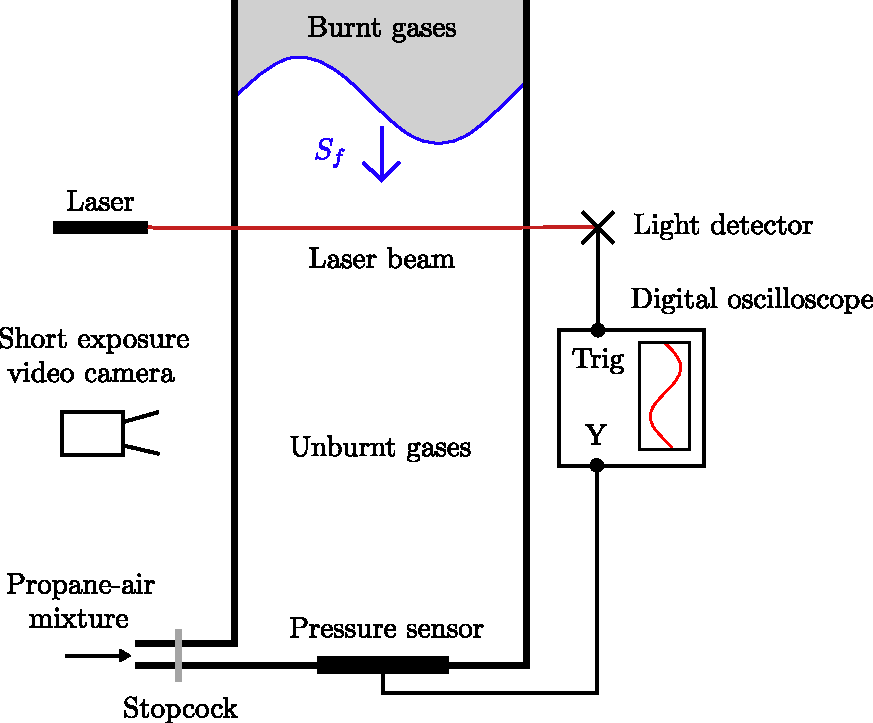
\includegraphics[scale=0.6]{assets/imgs/Searby-92.pdf}
\caption{Illustration of the experimental apparatus of \cite{searby1992AcousticInstabilityPremixed}.}
\label{fig:searby-experiment}
\end{figure}

An insightful experiment into thermoacoustics was performed later in 1992 by Searby \cite{searby1992AcousticInstabilityPremixed} and studied relationships between a cylindrical tube's acoustics as well as the speed and shape of the premixed flame within. The experimental apparatus is depicted in \fig{fig:searby-experiment}. Propane-air mixtures were lit at the top end of the tube and propagate down, with any acoustic disturbance detected by a pressure sensor at the bottom. Additionally, a small laser beam was place near the top of the tube to detect the flame as thermal gradients deflect the light. This triggers a digital oscilloscope to record pressure disturbances from the pressure sensor. A short exposure video camera was used to image the flame surface and observe its structure as it propagates. Since propane (C$_3$H$_8$) is a relatively heavy fuel with a species diffusion rate lower than methane's, the lean and stoichiometric mixtures used have Lewis numbers which are never below the critical Lewis number, $\Le_\rm{crit}$, required for \emph{thermodiffusive instabilities} \cite{zeldovich1944TheoryCombustionDetonation,barenblatt1962DiffusionalThermalStabilIty,sivashinsky1977DiffusionalThermalTheoryCellular} to have an effect. Note that the downward propagating flames will have been somewhat stabilised by the \emph{Rayleigh-Taylor} (RT) instability. The primary instability is observed alongside a secondary, which is associated with a different feedback mechanism, acoustic envelopes and flame dynamics.

\begin{figure}[t]
\centering
\begin{subfigure}{0.49\textwidth}
\centering
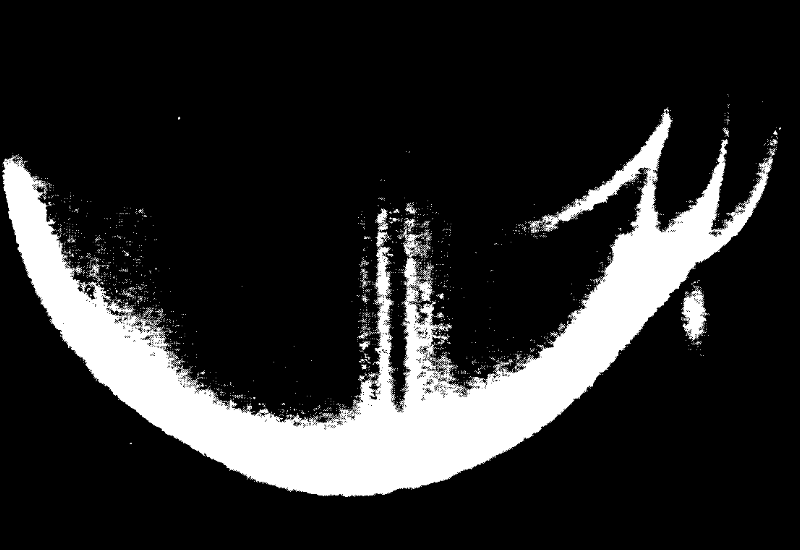
\includegraphics[height=5cm]{assets/imgs/Searby-92-flame_a.png}
\caption{}
\label{fig:Searby-92_flames_a}
\end{subfigure}
\hfill
\begin{subfigure}{0.49\textwidth}
\centering
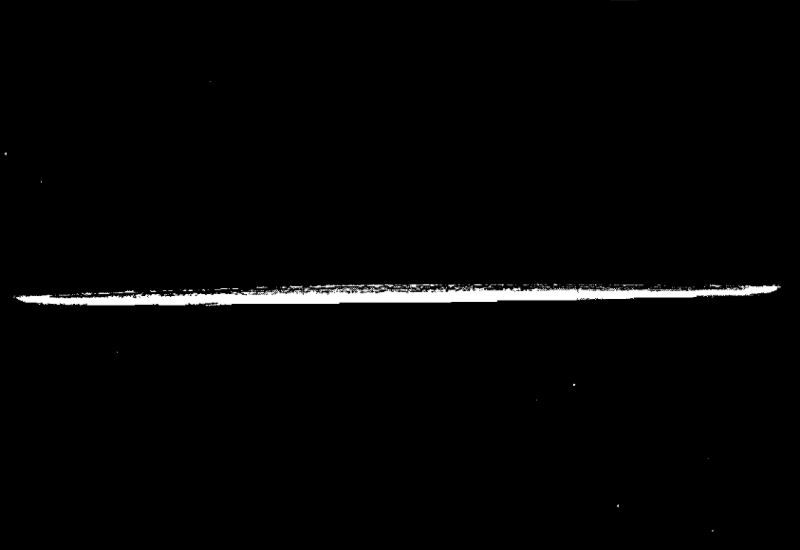
\includegraphics[height=5cm]{assets/imgs/Searby-92-flame_b.png}
\caption{}
\label{fig:Searby-92_flames_b}
\end{subfigure}

\vspace*{3mm}

\begin{subfigure}{0.49\textwidth}
\centering
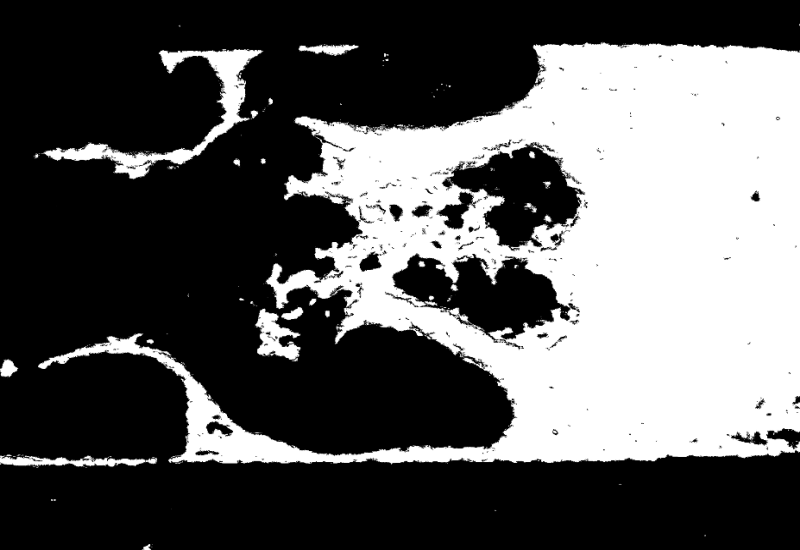
\includegraphics[height=5cm]{assets/imgs/Searby-92-flame_c.png}
\caption{}
\label{fig:Searby-92_flames_c}
\end{subfigure}
\hfill
\begin{subfigure}{0.49\textwidth}
\centering
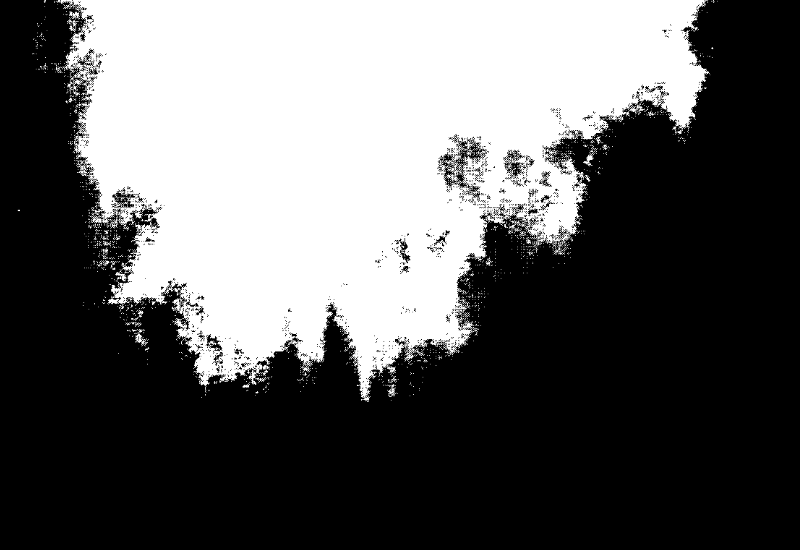
\includegraphics[height=5cm]{assets/imgs/Searby-92-flame_d.png}
\caption{}
\label{fig:Searby-92_flames_d}
\end{subfigure}
\caption{Photos, courtesy of \cite{searby1992AcousticInstabilityPremixed}, of flames at different stages of TA response. (a) shows the characteristic curved shape of a hydrodynamically unstable flame before any acoustics are significantly effecting the flame shape. (b) is a flame flame under the effect of the primary TA instability. (c) shows a cross-sectional slice of a flame rotated by $90\degree$ under the secondary instability. (d) shows a flame after the breakdown of cellular structures, which leads to a self-turbulent flame.}
\label{fig:Searby-92_flames}
\end{figure}

Initially, the flame curves as a result of the hydrodynamic instability, as photographed in \fig{fig:Searby-92_flames_a}. After some time, the acoustic amplitude increases due to primary instability. As the acoustic amplitude increases the flame flattens, seen in \fig{fig:Searby-92_flames_b}, resulting in a decrease in flame speed due to the decreased fuel consumption rate. In some of the flames tested, only the primary instability is observed, but in some others it progresses beyond this to the secondary instability -- often before the fully flattened flame is observed. At the immediate onset of the secondary instability, if it occurs, a cellular structure of a given wavenumber appears and corresponds to a rapid increase in the acoustic amplitude. This onset is much more rapid than for the primary instability, and eventually the cellular structure transitions into a symmetric flame structure similar to \fig{fig:Searby-92_flames_c}. Provided the flame has not yet reached the end of the tube it may also devolve into a self-turbulent flame similar to that shown in \fig{fig:Searby-92_flames_d}. The flame structures resulting from the secondary instability have significantly higher velocities as a result of their massively increased flame surface area and are viewed as a violent instability. The self-turbulent regime marks a significant decline to the acoustic amplitude as there is no regular release of pressure fluctuations from the flame.
% Flat flame under primary can be seen as a limit cycle

The secondary instability mechanism is seen by Searby \cite{searby1992AcousticInstabilityPremixed} as a \emph{parametric instability}. Searby and Rochwerger \cite{searby1991ParametricAcousticInstability} pose this system as a Mathieu equation by incorporating the effect of acoustic force into an equation for flame position under the influence of gravity, which is otherwise written as a damped harmonic oscillator \cite{searby1986WeaklyTurbulentWrinkled}. The Mathieu equation demonstrates a canonical example of parametric instability, since solutions remain unbounded whenever the forcing acoustic frequency is double that of the natural frequency implied by the flame in its damped harmonic oscillation. Physically this corresponds to a flame with a structure that oscillates with a period double that of the acoustic period.

% EXPLAIN WHAT S_L AND L_TH ARE
\begin{figure}[t]
\centering
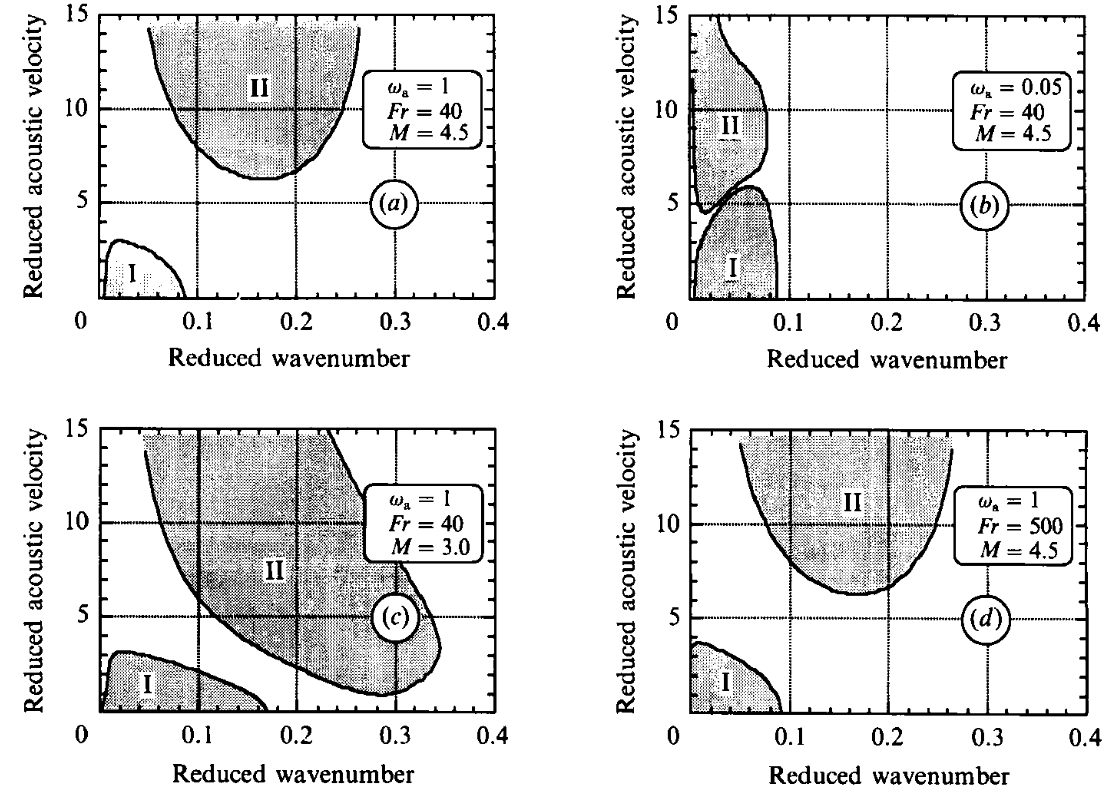
\includegraphics[height=11cm]{assets/graphs/thermoacoustic-stability.png}
\caption{Stability diagrams, courtesy of \cite{searby1991ParametricAcousticInstability}, for four different values of $ω_a$, $\Fr$ and $\Mk$. The regions I and II are regions of instability for the plane flame. Reduced wavenumbers are given as $k l_\rm{th}$ and reduced acoustic velocities are $u_a / S_L$.}
\label{fig:ta-stab}
\end{figure}

Using this formation of the flame front as solutions to the Mathieu equation, \cite{searby1991ParametricAcousticInstability} calculates regions of flame instability for a planar flame as functions of perturbation wavenumber $k$, acoustic velocity $u_a$ (the amplitude of which can be thought of as the intensity or volume of sound), acoustic frequency $ω_a$, Froude number $\Fr$ (representing non-dimensional inverse of gravitational forcing) and Markstein number $\Mk$ (a crucial flame parameter connecting the sensitivity of the flame's speed to perturbations to its surrounding hydrodynamics). They then plot these regions in \fig{fig:ta-stab}. Note that these plots do not acoustic instability mentioned above, but their effect on flame stability for a planar flame. In all the plots, there are two disjoint regions of flame instability. The region I represents hydrodynamic instability and occurs, as expected, at zero acoustic velocity for some wavenumber interval. This region ends at some finite $u_a$ as the primary acoustic instability eventually overcomes the hydrodynamic one. At non-zero acoustic velocity, region II of flame instability begins, corresponding to the aforementioned parametric instability. Interestingly, some of the graphs show acoustic velocities where regions I and II can coexist for different wavenumber intervals. In these cases, the primary thermoacoustic instability is expected to lead immediately into the secondary instability with no planar flame observed. On the other hand, for those acoustic velocities where neither region is present the planar flame is stable, so we see structures like \fig{fig:Searby-92_flames_b} where the flame has spontaneously flattened before any secondary instability can occur. We also notice that there is a wavenumber in region II which corresponds to the lowest unstable acoustic velocity. This means that once this acoustic velocity is met, only that wavenumber (and wavenumbers close to it) will be present as wrinkles in the flame. Finally, we note that the effect of increased gravity (decreased $\Fr$) on these downward propagating flames has stabilised the very low wavenumbers next to region I as the RT effect actually stabilises the plane flame.

An experiment was also performed by \cite{searby1991ParametricAcousticInstability} to demonstrate these results. A similar apparatus to \fig{fig:searby-experiment} was used, with significant changes being the usage of a loudspeaker in the bottom of the combustion tube to play sounds of wavelength one-quarter or three-quarters of the wavelength of the tube. A porous plate was placed above the loud speaker to remove any turbulence such that our laminar theories can be applied. Using the loud speaker to excite the flame at known volumes and frequencies (which correspond to controlling $u_a$ and $ω_a$, respectively), they observe both the planar and wrinkled flames described above. The sound intensity corresponding to the quietest parametrically unstable flame may then be plotted for a variety of acoustic frequencies, resulting in a curve predicted by the Mathieu equation model described above for a specific Markstein number. This enables the direct estimation of the Markstein number, which remains a difficult challenge and so remains a prevalent technique \cite{delfin2024ThermoacousticParametricInstability}.

Beyond this, TA oscillations have been observed in a variety of experimentation. Methane-air combustion in a cylindrical tube was investigated experimentally in \cite{fichera2001ExperimentalAnalysisThermoacoustic} with data recorded from an optical sensor to detect changes to heat release, a pressure transducer for internal pressure recordings and a microphone for external pressure recordings. TA oscillations were observed and a non-linear analysis into the dynamical behaviour of the flame recordings demonstrate a chaotic nature to these thermoacoustics. The global stability of the flame, which is guaranteed by diffusive effects, is corroborated via calculation of the set of Lyapunov exponents. The thesis \cite{ebieto2017DynamicsPremixedFlames}, provides a detailed setup to gather high-speed imagery, chemiluminescent and pressure data in a variety of TA flames. The effects of a variety of phenomena affecting acoustic stability, such as RT instability, are outlined. Further experimentation is done on premixed flame oscillations in \cite{delfin2024VideoTransientParametric,martinez-ruiz2018VideoPremixedflameOscillations,delfin2024ThermoacousticParametricInstability} and provide high-fidelity imagery of flames under the effects of primary and secondary instability in \cite{delfin2024VideoTransientParametric,martinez-ruiz2018VideoPremixedflameOscillations}.





\subsection{Thermoacoustic Instability Modelling}

\begin{figure}[t]
\centering
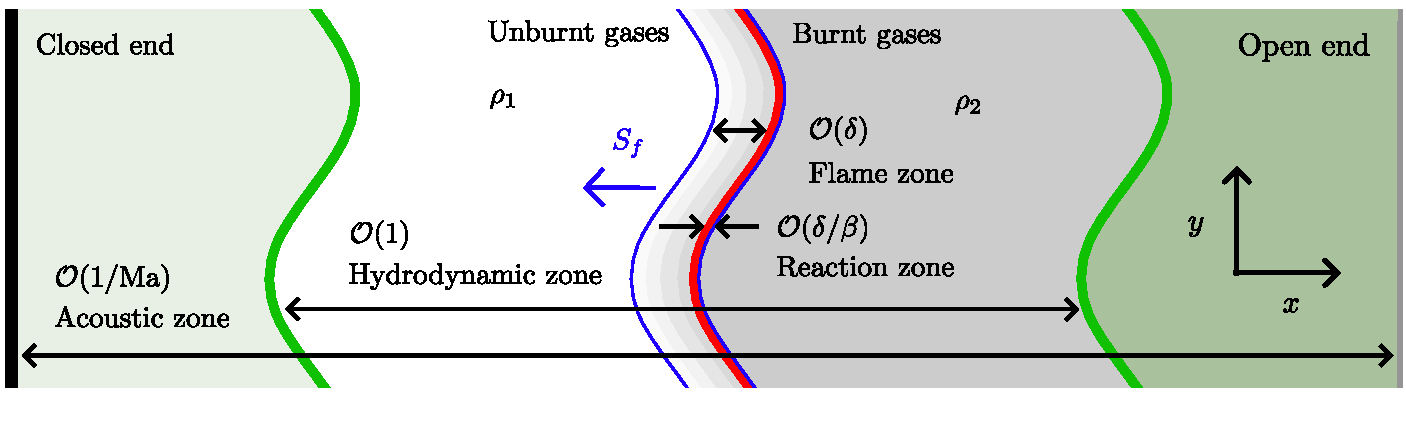
\includegraphics[scale=0.6]{assets/imgs/AW-flame.pdf}
\caption{Diagram showing the model geometry of the multiscale analysis performed by \cite{assier2014LinearWeaklyNonlinear}. The different non-dimensionalised asymptotic scales involved in the full analysis are labeled above the domain.}
\label{fig:AW-flame}
\end{figure}

Later on, work by Assier and Wu \cite{assier2014LinearWeaklyNonlinear} studied the stability of a \emph{flame-flow-acoustic} system, where a freely propagating flame in a closed-open, periodic duct is considered. \fig{fig:AW-flame} illustrates this geometry and is reminiscent of the experimental domain shown in \fig{fig:searby-experiment} of \cite{searby1992AcousticInstabilityPremixed}, excluding any wall boundary layer effects. Results from hydrodynamic flame theory \cite{matalon1982FlamesGasdynamicDiscontinuities,clavin1982EffectsMolecularDiffusion} are used to separate the dynamics within the flame from the outer fluid. This outer region is then separated into the usual $\cl{O}(1)$ hydrodynamic zone and a far-away $\cl{O}(1/\Ma)$ acoustic zone. Further asymptotic analysis is performed in the flame reference frame, coupling the two regions through dynamic jump conditions. A weak non-linearity assumption is made to simplify the flame equation such that linear stability analysis may be performed about the steady solutions to the Michelson-Sivashinsky equation \cite{sivashinsky1977NonlinearAnalysisHydrodynamic,michelson1977NonlinearAnalysisHydrodynamic,matalon2018DarrieusLandauInstability}.

They find that, when the acoustic interaction is included, these solutions are no longer linearly stable and the maximum growth rate of this instability increases significantly with heat release $q$. Non-linear stability analysis is also performed using a solver for the flame position coupled to the dynamical acoustic jump conditions. This is compared to the results of \cite{searby1992AcousticInstabilityPremixed} and they find they are able to qualitatively reproduce the primary instability and the onset of the secondary instability provided the flame parameter is allowed to deviate from its predicted value. In the latter case, the unsteady nature of the acoustic coupling to the flame induces an unsteady RT effect as the acoustic acceleration oscillates into and away from the less dense products. This is viewed as the driving mechanism behind this parametric instability. In a later conference paper, \cite{assier2014CombustionInstabilityModel}, tangential velocity terms are reintroduced and the parameter resulting in the same flame and acoustic behaviour as seen in \cite{searby1992AcousticInstabilityPremixed} more closely match the expected value. These results are surprisingly fruitful given they assume weak non-linearity in the face of the large heat releases the model is tested against.

In \cite{jun2023ParametricInstabilityPropagating} the secondary instability in hydrogen enriched methane-air flames is studied numerically in an open-ended tube. The structure of their flames under the full non-linear effect of the secondary instability is an impressive match to the experiment of \cite{ebieto2017DynamicsPremixedFlames}, in spite of a lack of convergence in the phase of sub-harmonic oscillations to the flame front (between grid spacings of 100 $μ$m to 50 $μ$m). They also find that the Rayleigh Index, $\rm{RI}$ is a good indicator for the onset of the secondary instability and that the violent acoustic output of this parametric instability may also be attributed to the changes in flame surface area strengthening oscillations in heat release which cause the thermoacoustic effect. They determine the main reason secondary instability is not seen in simulations of faster flames is simply that the tube is not long enough for the instability to develop before the flames reach the end of the tube. This validates a desire to model the behaviour of flames which are held in place, such as those in a held in place by combustor geometry in counterflow.


% veiga-lopez2020ThermoacousticAnalysisLean
% - Experimental study of H2-air flames in Hele-Shaw cells
% - Study effects of confinement due to cell geometry, gravity and mixture composition on thermoacoustic oscillations
% - Heat loss effects are most prevalent for very thin cells, where ...




\subsection{G-Equation Model}

% Aimee morgans




\subsection{Low-Order Thermoacoustic Modelling}

% n-tau models
% control theory stuff i don't understand

\cite{juniper2018SensitivityNonlinearityThermoacoustic}




\subsection{Instability Control}

\begin{figure}[t]
\centering
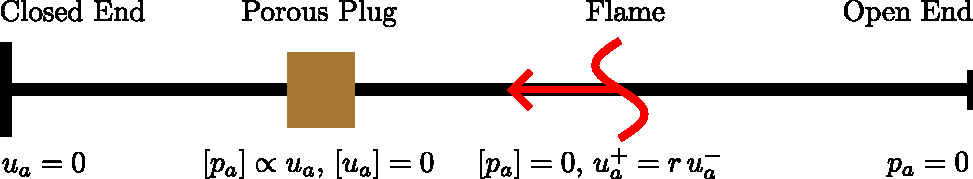
\includegraphics[scale=0.6]{assets/imgs/GP-model.pdf}
\caption{Illustration of the one-dimensional model considered by \cite{gaton-perez2025MitigationThermoacousticInstabilities}, where boundary conditions for each component of the model are shown.}
\label{fig:GP-model}
\end{figure}

Simpler analysis is performed by Gatón-Pérez et al. \cite{gaton-perez2025MitigationThermoacousticInstabilities} to evaluate the eigenstates of a one-dimensional closed-open tube containing a porous plug and a flame. Using Darcy's law to model the plug and assuming linear acoustics, the acoustic eigenmodes of the tube are found numerically. Experimental data is then compared against the one-dimensional model depicted in \fig{fig:GP-model}, where the heat release parameter, thermal length scale and the plug's permeability set by experimental values. Effects of heat losses through the combustor walls is given by \cite{flores-montoya2022NonadiabaticModulationPremixedflame}. The model is able to predict the flame locations within the tube which are most likely to trigger thermoacoustic resonance despite no consideration of the flame's motion or its thermal response to acoustics being made. These are the locations where the resulting acoustic eigenmodes have the lowest decay imposed by the porous plug. In this way, they show experimentally that the location of the porous plug may be chosen to preferentially mitigate different frequencies and reduce the likelihood of thermoacoustic instability. Evidently though, a simple one-dimensional model of this ilk is restricted in application to strongly one-dimensional, ducted combustors. As soon as a broader combustor or plenum is used, the two-dimensional acoustics (e.g. Helmholtz modes) must also be considered.

% luzzato2015ModellingControlCombustion (THESIS)

% liao2025ActiveControlThermoacoustic

% meadows2015PorousInsertsPassive

% mcmanus1993ReviewActiveControl




\subsection{Intrinsic Thermoacoustic Feedback}

\begin{figure}[t]
\centering
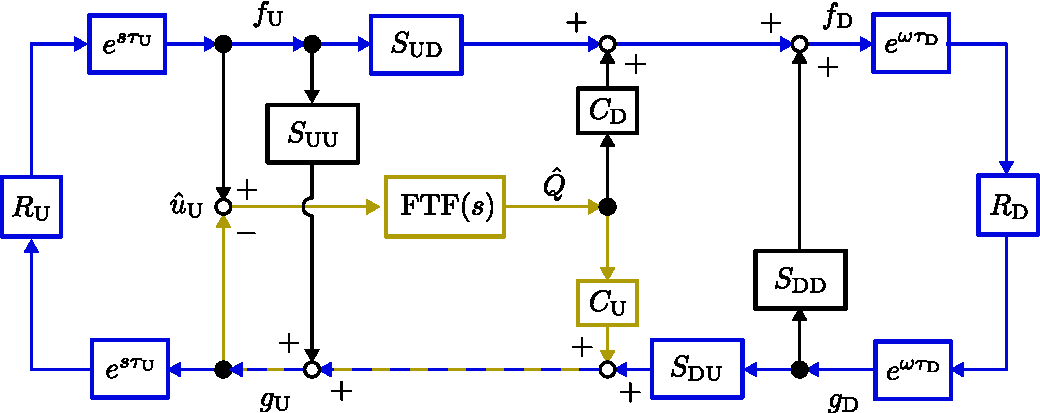
\includegraphics[scale=0.65]{assets/imgs/ITA-mech.pdf}
\caption{INTRINSIC THERMOACOUSTIC FEEDBACK LOOP}
\label{fig:ita-loop}
\end{figure}

% Doesn't need to be too elaborate!

% But there are not just acoustic modes, the full set of thermoacoustic instability modes includes ITA too [cite?]
% explain feedback loop
% phasors are cool
% some other stuff i read about
% cite the good reviews!

\cite{emmert2015IntrinsicThermoacousticInstability}
\cite{silva2023IntrinsicThermoacousticInstabilities}
\cite{hoeijmakers2014IntrinsicInstabilityFlame}
\cite{hoeijmakers2016FlameDominatedThermoacoustic}
\cite{orchini2025TrackingAcousticIntrinsic}
\cite{chen2024BiglobalLinearStability}
% Polifke?






\section{Techniques for Computational Fluid Dynamics (CFD)}

% Mention AVBP and CERFACS?

\cite{, domingo2023RecentDevelopmentsDNS, chen2011PetascaleDirectNumerical, yang2015LargeEddySimulationPresent, veynante2002TurbulentCombustionModeling, moin1998DirectNumericalSimulation, tennekes1972FirstCourseTurbulence}

The most brute force way to simulate a fluid system would be one where you try to accurately simulate every detail involved in the fluid. This idea was first studied by Orszag \cite{orszag1970AnalyticalTheoriesTurbulence}, where he defines \emph{direct numerical simulations} (DNS) as a numerical simulation with enough grid points to full resolve the smallest physical phenomena in the system. Originally, Orszag studied this in the context of turbulent flows. In turbulent flows, we have vortices not only on the order of the typical flow length scale $l_T$, called the integral length scale, but also of sizes all the way down to the smallest turbulence scale known as the kolmogorov length scale $l_K$ [CITE], where the rate at which viscous dissipation effects dampen vortices far exceeds the inertial forces of the vortex. In DNS of turbulent combustion, the smallest scale vortices must be resolved in addition to the smallest chemical length scales. In this context, the relevant time scales are chemical $τ_C = l_{\rm{th}} / S_L$, integral $τ_T = l_T / u'$ and Kolmogorov $τ_K = l_K / u'$ given an RMS velocity scale $u'$. Hence, the number of degrees of freedom required to resolve a three-dimensional box of size $L$ is:
\begin{equation}
N_{\rm{tot}} = \left( \frac{L}{2 l_T} \right)^3 \, \Da \, \Ka \, \rm{Re}_T^{7 / 4}
\end{equation}
where we define the turbulent Reynolds, Damköhler and Karlovitz numbers by:
\begin{equation}
\rm{Re}_T \equiv \left( \frac{l_T}{l_K} \right)^{4 / 3},
\quad
\Da \equiv \frac{τ_T}{τ_C}
\quad \text{and} \quad
\Ka \equiv \frac{τ_C}{τ_K}
\end{equation}
respectively.


For most turbulence intensities and combustion reactions, this means having a discretisation length scale on the order of 10 - 100 $μ$m.

% The size of this kolmogorov length scale is determined by the turbulent reynolds number and the integral scale with the relationship

% A consequence of this is the extraordinary computational cost to accurately simulate a large domain. To fully resolve DNS of turbulent combustion, for example, the small chemical length scale must be resolved in addition to the smallest scale vortices. 

% An alternative method that is widely used is LES and involves using models to estimate the transfer of energy at the smallest scale rather than fully simulating them [cite les review: Yang 2015]
% DNS for turbulent combustion are reviewed in \textbf{Domingo and Vervisch 2023} (with connection to LES) and \textbf{Chen 2011}.

% For small-scale, low-speed methane-air and hydrogen-air combustion, the flows we look at have similar properties to air, so are not very viscous meaning the smallest scale vortices in a fully developed turbulent may be ~...?
% But the turbulence usually isn't our biggest worry, since we also have the thin region that the reaction is taking place to resolve, usually only 300 {\textmu}m which is resolved with ~15 nodes in a high order code
% Regardless, when performing DNS careful consideration must be made to use ample sample points

% ?? DNS with simple transport / chemical schemes?

\subsection{Mesh-free Methods}

\cite{monaghan1992SmoothedParticleHydrodynamics, vacondio2021GrandChallengesSmoothed}





\subsection{High-Order Discretisation}




\subsection{Navier-Stokes Characteristic Boundary Conditions}

\cite{thompson1987TimeDependentBoundary, thompson1990TimeDependentBoundaryConditions, poinsot1992BoundaryConditionsDirect, poinsot2005TheoreticalNumericalCombustion, sutherland2003ImprovedBoundaryConditions}

% [Thompson 1987, 1990, Poinsot and Lele 1992, Sutherland and Kennedy 2003, Poinsot and Veynante 2005]


% Many types of boundary conditions may be chosen for combustion schemes:
%% Periodic are very simple to enforce numerically so require no elaboration
%% No-slip or slip wall conditions
%% isothermal or adiabatic walls
%% acoustically reflecting or non-reflecting walls or inflow / outflow
%% In the case of inflow / outflow many more cases

% In most of these cases, we can use the formalism called characteristic boundary conditions (characteristic BCs)




% The simplest boundary conditions, i.e. those with constant (Dirichlet) boundary values (p=const), usually reflect acoustic waves back toward the interior of the domain. For most situations we want to simulate, this doesn't represent the physical situation, where we would rather pretend the medium continues outside of the computational domain. This motivates a need for boundary conditions which do not reflect acoustic waves - non-reflecting boundary conditions. The formalisms are based of characteristic waves entering / leaving the domain

% Fixed velocity inlets give full reflections, so cannot be used in a non-reflecting case.

% Immersed boundary methods are also an option and open up possibilities for boundaries not restricted specific node placement, especially for moving boundaries. But as detailed in King 2022, these a largely restricted to lower order accuracy at these boundaries (cite, and for what reason?).



\subsection{Delayed-Time Domain Impedance Boundary Conditions}


% Describe TDIBC briefly before going into time delay model!


\begin{figure}[t]
\centering
\includegraphics[scale=0.65]{example-image-a}
\caption{D-TDIBC}
\label{fig:D-TDIBC}
\end{figure}

Although many variations on TDIBC exist, the \emph{Delayed-Time Domain Impedance Boundary Conditions} (D-TDIBC) of \cite{douasbin2018DelayedtimeDomainImpedance} are particularly relevant for the simulation of thermoacoustic instabilities. By modelling the effect of an acoustic time delay, $τ$, a part of the computational domain -- say, an exhaust pipe -- may be truncated in place of a numerical boundary. Then, the response of this new boundary to incoming acoustics should be a sinusoidal Moiré pattern in the frequency domain. The proposition of \cite{douasbin2018DelayedtimeDomainImpedance} is that this pattern may be modelled via a meromorphic function of $2n$ simple poles. The location of these poles and their residues are then found in a preprocessing step as the values which minimise the least-squares fit with the desired response curve. Each time step then, the resulting constants are used to evaluate the change in acoustic variable at the boundary in such a way that no memory of previous time steps are required. 

After validating the model by testing its response to a Gaussian pressure bump, the model is compared against DNS of methane-air combustion in a 2D flame holder, where the upstream end is closed and the downstream end is open. Comparing this to DNS where the last 25 cm at the downstream end has been truncated to use D-TDIBC, they find that the time delay model accurately recovers the one-, three- and five-quarter eigenmode shapes, with small quantitative errors in their sound spectra. Considering the $\sim 13\%$ reduction in degrees of freedom in the computational domain resulting from the truncation, this can be seen as an impressive recovery of the problem's physics by using what is essentially a one-dimensional low-order model in the truncated region for the acoustics. Since the model constants are calculated as a preprocessing step, the envelope of the acoustic response in the frequency domain may essentially be changed arbitrarily, presenting a benefit in case different pass bands are desired.

Besides the inevitable drawbacks stemming from: the low-order model's inaccuracy and the requirement of a strongly one-dimensional flow at the boundary to match this model, other drawbacks remain prevalent. For one, no method to visualise acoustics residing in the fictitious, truncated domain is provided, potentially leading to a \emph{black-box} of energy where acoustics are essentially stored, but not known. For another, the preprocessing steps are required for each value of $τ$ used. So, if the time delay were to change dynamically during the simulation (e.g. due to an expanding computational domain to ensure the flame remains within), this preprocessing may happen each step, becoming computationally costly.







\chapter{Markstein Model Calculations} \label{ch:markstein}
\section{Theory}


\begin{figure}[t]
    \centering
    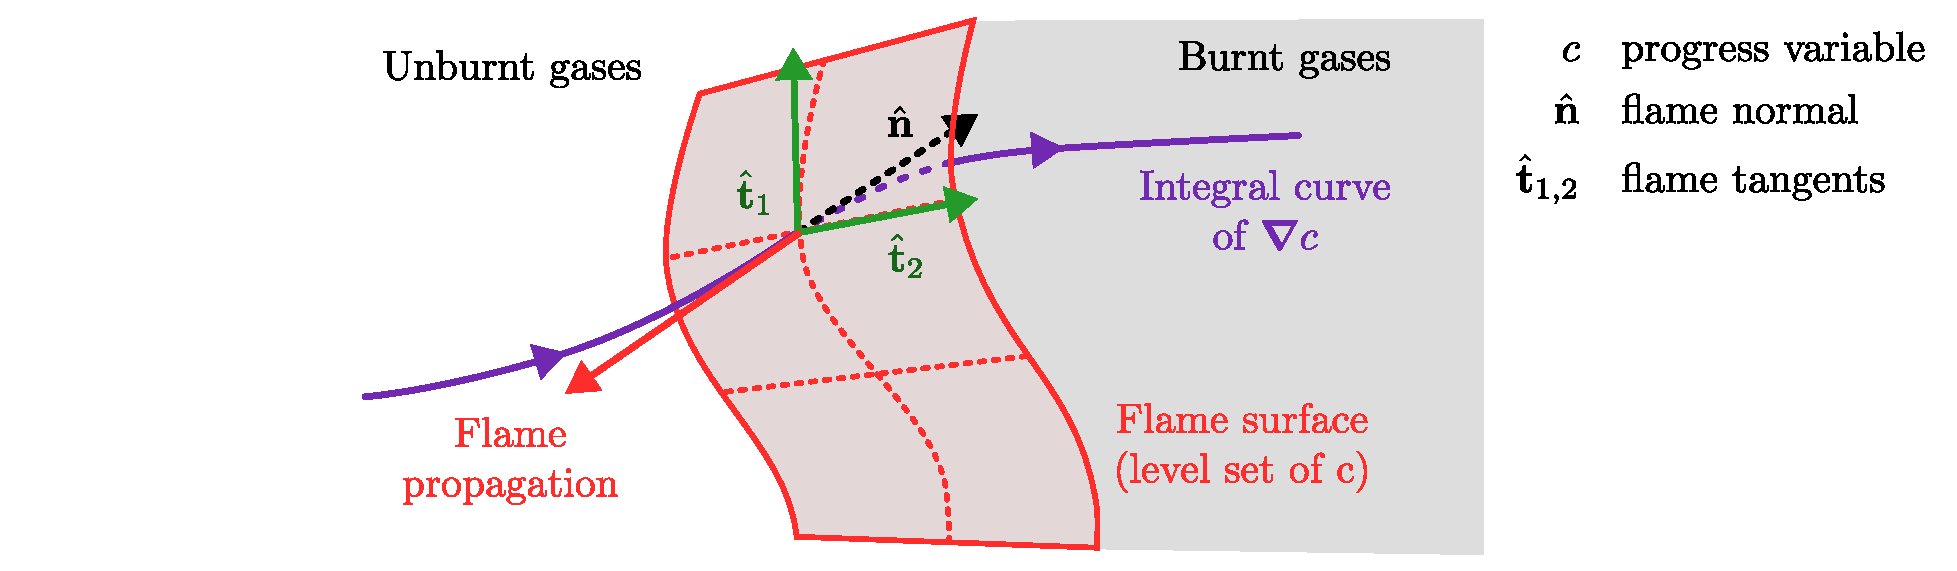
\includegraphics[scale=0.43]{assets/imgs/flamelet.pdf}
    \label{fig:flamelet}
    \caption{Diagram of the 3D flame surface model used below.}
\end{figure}

Defining the inverse thermal Peclet number: $\d = l_\rm{th} / L$ as the asymptotic parameter used by \cite{pelce1982InfluenceHydrodynamicsDiffusion,matalon1982FlamesGasdynamicDiscontinuities} to describe flame thickness alongside the Zeldovich number $\Ze$ which loosely prescribes reaction zone thickness relative to the flame thickness, the work of \cite{pelce1982InfluenceHydrodynamicsDiffusion,matalon1982FlamesGasdynamicDiscontinuities} primarily finds that the incompressible Navier-Stokes (NS) equations are suitable approximations of gas flow on either side of a premixed deflagration which is deficient in one reactant:
\begin{subequations}
\begin{boxaliat}{2}
\label{eqn:hydro-incomp} \vec{\nabla}\cdot\vec{u} &= 0                         &&+ \cl{O}\left( \d^2 \right), \\
\label{eqn:hydro-u} \r \mdv{\vec{u}}{t} &= - \vec{\nabla}p + \d\Pr \lap\vec{u} &&+ \cl{O}\left( \d^2 \right).
\end{boxaliat}
\end{subequations}
So these equations are valid on either side of the flame, which we describe mathematically by the level set of a function $F = 0$. The asymptotic papers make the additional assumption that this level set looks like the graph of a function in $y$, $f(y, t)$, such that e.g. in two-dimensions $F \equiv x - f(y, t)$. For numerical purposes, it is usually easiest to define this level set via the progress variable:
\begin{equation}
c \equiv \frac{Y_\a - Y_{\a, 1}}{\bbra{Y_\a}_V}
\end{equation}
for one of the species $\a$, so $F \equiv c - c^*$. The graph assumption is not the case for flames typically, so we instead rely on the level set formulation.

The \emph{product-pointing} normal (i.e. the normal which points towards the hot, light reaction products) is easily defined by:
\begin{equation}
\uvec{n} \equiv \frac{\vec{\nabla}c}{\norm{\vec{\nabla}c}} \bigg|_{F^-}.
\end{equation}
which is the unit normal vector pointing forward along the integral curve of $\vec{\nabla} c$ which goes through the relevant point at the flame surface. The reactant-pointing normal may also be used, which just results in a change in sign. We use the product-pointing normal so we start off without negatives. The absolute speed of the flame at a point on the flame is the component of the flame motion $\ndt{\vec{f}}$ which moves away from the products:
\begin{subequations}
\begin{equation}
S_a \equiv - \ndt{\vec{f}} \cdot \uvec{n},
\end{equation}
and the displacement speed also considers the effect of the fluid moving at the products, opposing flame motion:
\begin{equation}
S_d \equiv (\vec{u} - \ndt{\vec{f}}) \cdot \uvec{n} \,\big|_{F^-} = S_a + \vec{u} \cdot \uvec{n} \,\big|_{F^-}.
\end{equation}
Hence, considering the advection equation for the flame: $\partial c / \partial t + \ndt{\vec{f}}\cdot \vec{\nabla}c = 0$ we find the following simple expressions for absolute and displacement speed:
\begin{align}
S_a &= \frac{1}{\norm{\vec{\nabla}c}} \pdv{c}{t} \,\bigg|_{F^-} \\
S_d &= \frac{1}{\norm{\vec{\nabla}c}} \mdv{c}{t} \,\bigg|_{F^-}
\end{align}
In this context, the species conservation equation may be used:
\begin{align}
\r \mdv{c}{t} &= \frac{1}{\bbra{Y_\a}_V} \cdot \r \mdv{Y_\a}{t} = \frac{1}{\bbra{Y_\a}_V} \left( \ndt{\vr}_\a - \vec{\nabla} \cdot (\r \vec{V}_{\!\a} Y_\a) \right), \\
\implies \quad \Aboxed{ S_d &= \frac{1}{\r \norm{\vec{\nabla}c} \bbra{Y_\a}_V} \left[ \ndt{\vr}_\a - \vec{\nabla} \cdot (\r \vec{V}_{\!\a} Y_\a) \right] \bigg|_{F^-} . }
\end{align}
\end{subequations}

It was primarily the work of Markstein in his seminal papers \cite{markstein1951ExperimentalTheoreticalStudies,markstein1953InstabilityPhenomenaCombustion,markstein1964NonsteadyFlamePropagation} which brought forth the idea that changes in flame speed away from its \emph{unstretched} speed, the laminar flame speed, is proportional to the amount of stretching that the flame experiences. Although Markstein first suggested a simple relationship between flame speed and curvature, it is now accepted that, at least in the hydrodynamically unstable regime, a dependence with the full \emph{flame stretch} is required. The dimensional and non-dimensional forms of these relations for consumption and displacement speed therefore follow: 
\begin{subequations}
\begin{alignat}{4}
S_{c/d}   &= S_L &&+ l_\rm{th} \Mk_{c/d}&&( -\bb{K}   &&) \\
S_{c/d}^* &= 1   &&+        \d \Mk_{c/d}&&( -\bb{K}^* &&)
\end{alignat}
\end{subequations}
with $\bb{K}$ being the flame stretch as elaborated in \cite{matalon1982FlamesGasdynamicDiscontinuities,candel1990FlameStretchBalance,clavin1985DynamicBehaviorPremixed}. This flame stretch obeys the formula:
\begin{subequations}
\begin{align}
(-\bb{K}) &= S_a (\vec{\nabla}\cdot\uvec{n}) + \uvec{n} \cdot \vec{\nabla} \cross (\vec{u}\cross \vec{n}) \Big|_{F^-} \\
&= S_d (\vec{\nabla}\cdot\uvec{n}) + \left[ (\uvec{n}\otimes\uvec{n}) : \vec{\nabla}\vec{u} - \vec{\nabla} \cdot \vec{u} \right] \Big|_{F^-} \\
&= S_d (\vec{\nabla}\cdot\uvec{n}) + \left(\uvec{t}_1\otimes\uvec{t}_1 + \uvec{t}_2\otimes\uvec{t}_2\right) : \bb{E} \,\Big|_{F^-} \\
&= S_d \kappa + E
\end{align}
\end{subequations}
depending on the flame's displacement speed, curvature $\k$ and strain $E$:
\begin{subequations}
\begin{align}
\kappa &\equiv \vec{\nabla}\cdot\uvec{n}, \\
E &\equiv \left(\uvec{t}_1\otimes\uvec{t}_1 + \uvec{t}_2\otimes\uvec{t}_2\right) : \bb{E} \,\Big|_{F^-} = \left[ (\uvec{n}\otimes\uvec{n}) : \vec{\nabla}\vec{u} - \vec{\nabla} \cdot \vec{u}\right] \, \Big|_{F^-}, \\
\bb{E} &= \frac{1}{2}\left(\vec{\nabla}\vec{u} + (\vec{\nabla}\vec{u})^T\right)
\end{align}
where $\bb{E}$ is the strain rate tensor and the vectors $\uvec{n}$, $\uvec{t}_1$ and $\uvec{t}_2$ form a moving frame on the flame surface (assuming a three-dimensional system):
\begin{equation}
\uvec{t}_{1, 2} \cdot \uvec{n} = 0
\quad \text{and} \quad
\uvec{t}_{1} \cdot \uvec{t}_2 = 0.
\end{equation}
\end{subequations}
Finally, the values $\Mk_{c/d}$ are the \emph{Markstein numbers} for the consumption and displacement speed of the flame. Classic formulae used for these values are known as the \emph{Clavin-Williams formulae} \cite{clavin1982EffectsMolecularDiffusion}:
\begin{subequations}
\begin{alignat}{2}
\Mk_d &= \Mk_1 + && \frac{1}{2}\Ze (\Le - 1) \Mk_2, \\
\Mk_c &=         && \frac{1}{2}\Ze (\Le - 1) \Mk_2,
\end{alignat}
\end{subequations}
placeholder
\begin{subequations}
\begin{alignat}{2}
\Mk_1 &\equiv \frac{1 + q}{q} \ln (1 + q)             && > 0, \\
\Mk_2 &\equiv \int_{-\infty}^0 \ln (1 + q e^x) \dd{x} && > 0.
\end{alignat}
\end{subequations}


% jump conditions (use matalon independent flame equations)
% enhancement factors
% Local flame speeds etc.
% integral curves, contours and averaged vs summed local speeds




\section{Methodology}

\begin{figure}[t]
    \centering
    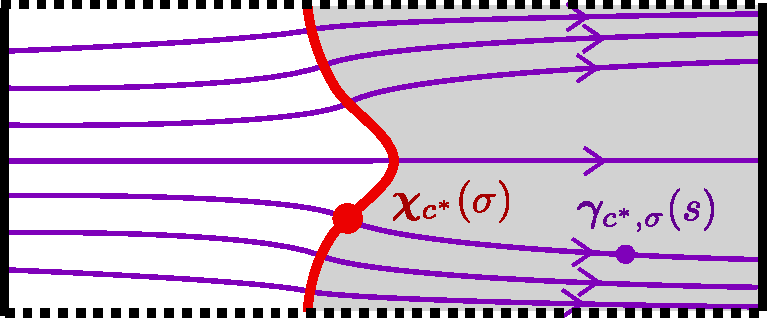
\includegraphics[scale=0.43]{assets/imgs/2d-flame-int-curves.pdf}
    \label{fig:int-curves}
    \caption{caption}
\end{figure}

These are sets depending on time, $t$, which we ignore below for brevity
\begin{subequations}
\begin{alignat}{2}
\chi_{c^*}       &\equiv \Big\{ \vec{\chi}_{c^*}(\sigma)  \, &&| \  c\big(\vec{\chi}_{c^*}(\sigma)\big) = c^* \Big\} \\
\g_{c^*, \a} &\equiv \Big\{ \vec{\g}_{c^*, \s}(s) \, &&| \  \vec{\g}_{c^*, \s}' =  \vec{\nabla}c / \norm{\vec{\nabla}c} \big|_{\vec{\g}_{c^*, \s}} \ \text{and} \  \vec{\g}_{c^*, \s}(0) = \vec{\chi}_{c^*}(\sigma) \Big\}
\end{alignat}
\end{subequations}
we find that the set integral curves does not change with time or the contour progress variable $c^*$ and covers domain:
\begin{subequations}
\begin{align}
A &= \big\{ \vec{\g}_{c_1, \s_1}(s_1) \, | \ s_1, \ \s_1 \ \text{and} \ \vec{\g}_{c_1, \s_1} \in \g_{c_1, \s_1} \big\} \\
&= \big\{ \vec{\g}_{c_2, \s_2}(s_2) \, | \ s_2, \ \s_2 \ \text{and} \  \vec{\g}_{c_2, \s_2} \in \g_{c_2, \s_2} \big\}
\end{align}
\end{subequations}
where $c_1 \neq c_2$. This ensures that integral quantities over the whole domain $A$ are exactly calculated by the continuous summation of integrals of the same quantity over each integral curve. For consumption speed $S_c$, this means that:
\begin{equation}
S_{c, \rm{loc}}(\s) = \frac{1}{\r_1 \bbra{T}_A} \int_{s_1}^{s_2} \frac{\ndt{\cl{T}}(\s, s)}{c_p(\s, s)} \dd{s},
\quad \text{and} \quad
\overline{S_{c, \rm{loc}}} = \frac{1}{L[\chi]} \int_{\s_1}^{\s_2} S_{c, \rm{loc}}(\s) \dd{\s}
\end{equation}
so
\begin{subequations}
\begin{align}
S_c &= \frac{1}{w \r_1 \bbra{T}_A} \int_A \frac{\ndt{\cl{T}}}{c_p} \dd{A} = \frac{1}{w \r_1 \bbra{T}_A} \int_{\s_1}^{\s_2} \int_{s_1}^{s_2} \frac{\ndt{\cl{T}}(\s, s)}{c_p(\s, s)} \dd{s} \dd{\s} \\
&= \frac{1}{w} \int_{\s_1}^{\s_2} S_{c, \rm{loc}}(\s) \dd{\s} = \frac{L[\chi]}{w} \cdot \overline{S_{c, \rm{loc}}}
\end{align}
\end{subequations}

% This means that integral quantities over the whole domain (S_c) can be exactly calculated through integrals over the curve of the same integral values (S_c,loc) over individual integral curves
% For S_c this turns out to be: integral over area = integral over x then y = integral over integral curve then contour

% Our contour finding algorithm is the marching squares algorithm which, as the name suggests, requires a cartisian grid of input data. We interpolate our unstructured mesh-free nodes onto a cartesian grid using cubic splines. Analyse only the DNS nodes which are in a rectangle around the flame so as to be non-negligible to same computational time. The contours may then be found for any progress variable c^*. The chemical progress variable c_Y was chosen here for the same reasons as Day et al and Howarth 2022 to better represent flame locations and reduce closed loop contours (C_Y = C_T FOR IDEALISED FLAMES, THEY HAVE NON-IDEALISED FLAMES). Note that the choice of the flame location is entirely arbitrary as a function of a continuous progress variable (in the asymptotic regime we essentially have discontinuous progress variable c = 0, the reactants, and c = 1, the products) so we are forced to make some sensible choice. we call this choice the flame progress variable c_flame, and take it to be a value of progress variable which best represents the location of highest heat release. Any other 'metric' could be used justifiably, and we hope at this stage that the value of the Markstein number is independent of this choice
% On this flame contour, normals may be calculated by travelling short distances along integral curves and used to calculate rate of strain and curvature. To calculate curvature we use a two point finite difference stencil:

% Rate of strain is calculated by the formula ( -- ) where spatial derivatives are easily calculated on the interpolated data via finite differences on the mesh points. Theoretically, rate of strain is evaluated just ahead of the flame, at f^-. In the context of simulation data this is again ambiguous as above, so we must choose its location. Normals are already treated to represent the shape of the flame, but for the upstream hydrodynamics, we must use some other metric. Hence, we choose to use a smaller progress variable, more representative of the reactant mixture location at the beginning of reaction, c_up. Rate of strain and all other evaluations of u will take place at the intersection of the c = c_up contour and the relevant integral curve. Note that we could instead evaluate values using a threshold density, but this is equivalent to using a temperature-based progress variable value.

% Flame thicknesses may be evaluated for each integral curve too. In Howarth and Aspden 2022 they have strong turbulence effects so the flame thickness vary significantly between integral curves. For these idealised laminar flames, however, we find that the flame thicknesses do not change significantly (1% or something?) so diffusive thicknesses are used unlike Howarth

% Displacement speed may be evaluated as in the previous section (equation 20f), but the evaluation of diffusive fluxes from the interpolated data generates spurious noise. Instead, we evaluate S_d from S_d = S_a + u . n. S_a may be simply estimated at steady states by assuming f dot is travelling horizontally, so then fdot = (u_in - S_c)e_x hat and ... 


% The mixing of u on upstream and n on flame contours may seem dubious, but actually when we do this our regression improves, justifying it quantitatively



\section{Results}





\chapter{Combustion Simulation Techniques} \label{ch:techniques}


\section{LABFM}

\cite{king2024MeshFreeFrameworkHighOrder, king2020HighOrderDifference, king2024MeshfreeFrameworkHighorder, king2022HighorderSimulationsIsothermal, king2024SunsetFlamesDNSCode}


\subsection{High-Order Interpolations}

% in keeping with other methods, where interpolation is the first step to gradient approximations

Before considering gradient approximations, we first consider interpolations, hoping that they are simpler and elucidate a method for us. We consider a location $\vec{x}$ surrounded locally by finitely many nodes $\vec{x}_j \in \cl{S}(\vec{x})$ which are enumerated by $j \in \cl{N}(\vec{x})$, where $\abs{\vec{x} - \vec{x}_j} < h(\vec{x})$ and a function $\phi = \phi(\vec{x})$ which is \emph{smooth enough}.\footnote{Some elaboration.} Then we express the interpolated value $\phi(\vec{x})$ as a linear combination of the surrounding function values $\phi_j = \phi(\vec{x}_j)$:
\begin{equation} \label{eqn:L}
L^{\rm{int}}[\phi](\vec{x}) \equiv \sum_{j \in \cl{N}(\vec{x})} \phi_j w^{\rm{int}}(\vec{x}, \vec{x}_j) \approx \phi(\vec{x}).
\end{equation}
To find the weights $w^{\rm{int}}(\vec{x}, \vec{x}_j)$, we must observe the contribution of function derivatives into $\phi$ by means on Taylor series. This derivative space is expressed as projections of the vectors of derivatives of $\phi$:
\begin{equation}
\vv{D}[\phi] = \left(\phi, \pdv{\phi}{x}, \pdv{\phi}{x}, \pdv[2]{\phi}{x}, \pdv[2]{\phi}{x}{y}, \pdv[2]{\phi}{x}, \dots \right)^T
\quad \text{and} \quad
\vv{D}_k[\phi] = \left(\phi, \pdv{\phi}{x}, \pdv{\phi}{x}, \dots, \pdv[k]{\phi}{x}, \dots, \pdv[k]{\phi}{y} \right)^T,
\end{equation}
where we have assumed that $\phi$ is a scalar field over two spatial dimensions $\vec{x}=(x, y)$, although the method may be simply extended to any number of dimensions. In this notation, interpolation is just $\phi(\vec{x}) = \vv{D}[\phi](\vec{x}) \cdot \vv{C}^{\rm{int}} = \vv{D}_k[\phi](\vec{x}) \cdot \vv{C}_k^{\rm{int}}$ where $\vv{C}^{\rm{int}} = (1, 0, 0, 0, 0, 0, \dots)^T$ and $\vv{C}_k^{\rm{int}} = (1, 0, 0, \dots, 0,)^T$, which is of the same length as $\vv{D}_k$. Then, upon introducing vectors of monomials:
\begin{equation}
\vv{X}(\vec{x}) = \left(1, x, y, \frac{1}{2!} x^2, xy, \frac{1}{2!} y^2, \dots \right)^T
\quad \text{and} \quad
\vv{X}_k(\vec{x}) = \left(1, x, y, \dots, \frac{1}{k!} x^k, \dots, \frac{1}{k!} y^k \right)^T,
\end{equation}
we can simplify down the Taylor expansion of $\phi$ around the point $\vec{x}$ for any $\vec{x}_j$ as:
\begin{subequations}
\begin{align}
\phi_j &= \phi(\vec{x}) + \pdv{\phi}{x}\bigg|_{\vec{x}} (x_j - x) + \pdv{\phi}{y} \bigg|_{\vec{x}} (y_j - y)  \\
& \qquad  \quad \ \, + \frac{1}{2!} \pdv[2]{\phi}{x}\bigg|_{\vec{x}} (x_j - x)^2 + \pdv[2]{\phi}{x}{y}\bigg|_{\vec{x}} (x_j - x) (y_j - y) + \frac{1}{2!} \pdv[2]{\phi}{y}\bigg|_{\vec{x}} (y_j - y)^2 + \dots \\
&= \vv{D}[\phi](\vec{x}) \cdot \vv{X} (\vec{x}_j - \vec{x}),
\end{align}
\end{subequations}
which may be truncated to $\phi_j \approx \vv{D}_k[\phi](\vec{x}) \cdot \vv{X}_k (\vec{x}_j - \vec{x})$ with $\cl{O}(h^{k + 1})$ truncation error. Rewriting \equ{eqn:L} in this formulation:
\begin{subequations}
\begin{align}
L^{\rm{int}}[\phi](\vec{x}) &= \vv{D}[\phi](\vec{x}) \, \cdot \sum_{j \in \cl{N}(\vec{x})} \vv{X} (\vec{x}_j - \vec{x}) w^{\rm{int}}(\vec{x}, \vec{x}_j) \\
&\approx \vv{D}_k[\phi](\vec{x}) \, \cdot \sum_{j \in \cl{N}(\vec{x})} \vv{X}_k (\vec{x}_j - \vec{x}) w^{\rm{int}}(\vec{x}, \vec{x}_j) \equiv \vv{D}_k[\phi](\vec{x}) \cdot \vv{B}_k^\rm{int}(\vec{x}) \\
&\approx \vv{D}_k[\phi](\vec{x}) \cdot \vv{C}_k^{\rm{int}}
\end{align}
\end{subequations}
So our problem now involves finding the correct values of $w^{\rm{int}}(\vec{x}, \vec{x}_j)$ such that the \emph{vector of moments} $\vv{B}_k^{\rm{int}}(\vec{x})$ of $w^{\rm{int}}$ approximates $\vv{C}_k^\rm{int}$. For consistency then, we require that the first component is independent of $h$:
\begin{equation}
1 = C_k^{\rm{int}, 0} \approx B_k^{\rm{int}, 0}(\vec{x}) = \sum_{j \in \cl{N}(\vec{x})} w^{\rm{int}} (\vec{x}, \vec{x}_j),
\end{equation}
so $w^{\rm{int}} = \cl{O}(h^0)$, where the superscript zeroes represent the leading vector component. The resulting error in this approximation is $\cl{O}(h^{k + 1})$, coming from the combined error from truncating the Taylor expansion of $\phi_j$ and approximating $w^{\rm{int}}$.

What's left is to find the weights of $w^{\rm{int}}$ in a way which can be solved for at any point $\vec{x}$ surrounded by nodes $\vec{x}_j$. To do this, we separate $w^{\rm{int}}$ into some anisotropic dependence of $\vec{x}$ on the surrounding nodes from the contribution that the action of interpolation has. This is done by writing it as the weighted sum of some anisotropic basis functions:
\begin{equation}
w^{\rm{int}}(\vec{x}, \vec{x}_j) = \vv{W}_k(\vec{x}_j - \vec{x}) \cdot \vv{\Psi}_k^{\rm{int}}(\vec{x})
\end{equation}
where the anisotropy is seen in the dependence of $\vv{W}_k$ on $(\vec{x}_j - \vec{x})$, which includes directional information, rather than $|\vec{x}_j - \vec{x}|$ (contrasting to the radial basis function method). Assuming that $\vv{W}_k$ comprises some known \emph{anisotropic basis functions} (ABFs) [we can find them according to king 2022], we must find the vector of weights $\vv{\Psi}_k^{\rm{int}}(\vec{x})$. This is done by substituting the new form into the vector of moments:
\begin{align}
\vv{C}_k^\rm{int}
\approx \vv{B}_k^{\rm{int}}(\vec{x})
= \left( \sum_{j \in \cl{N}(\vec{x})} \vv{X}_k (\vec{x}_j - \vec{x}) \otimes \vv{W}_k(\vec{x}_j - \vec{x}) \right) \cdot \vv{\Psi}_k^{\rm{int}}(\vec{x})
\equiv M(\vec{x}) \cdot \vv{\Psi}_k^{\rm{int}}(\vec{x})
\end{align}
where $M$ is a $n \times n$ matrix and $n$ is the number of components of $\vv{C}_k^\rm{int}$. The vector of weights $\vv{\Psi}_k^{\rm{int}}(\vec{x})$ is found when the linear system is solved. Carrying over the error terms from previous steps, we expect convergence on the order $\cl{O}(h^{k + 1})$.

% we require a number of nodes to ensure the linear system has a solution. typically the kernel is non-trivial, so we just need one solution
% The number of nodes required per stencil ~70 in 2D makes it expensive to calculate the weights for a given position to interpolate to. If you know beforehand where to interpolate to, this becomes cheap as it is done in preprocessing

% Cannot yet show convergence information unless I code this stuff myself (which I don't want to do)

% Stability?

% M condition number???? (worth mentioning but not extensively)


\subsection{High-Order Derivatives}

% Like other methods, we may wish to use this method of interpolation to find gradients as well. For classical methods, this is essentially done by differentiating the formulae we have already found. For LABFM, we have the benefit of a formulation where we can simply search for solutions where C = (0, 1, 0, ..) 
% For use in PDEs, we want gradients at points we have phi_i information at, so x becomes one of the nodes
% Since we are looking for derivatives now, we no longer require information on the absolute value phi_j, but the scalar relative to its value at the centre, phi_ji. The only change to the analysis above is that vectors e.g. X = (1, x, x^2/2, ...) -> X = (x, x^2/2) since the value phi_i = D[phi](x_i)^0 X(x_j - x_i)^0 is not needed
% Show new 'formula' and write in discrete notation X_ji not X(x_j - x_i)

% Ending - COST: we can do this process in any number of dimensions, although the cost scales rapidly from 2D to 3D as many more nodes x_j are contained within stencils. Usually have 70-80 nodes per stencil in 2D, making it quite expensive
% good part is that finer geometries are easy to resolve by scattering nodes. Mention how boundaries are discretised with 5 layers of nodes for upwinded finite differencing for outgoing waves
% Lagrangian methods are hard as above





% \blue{

% $$f(x) = y,\quad \text{also}, \quad \overset{\rightsquigarrow}{C}$$

% How do mesh-free methods help us generally, and what does LABFM do which is especially helpful? Mesh-free methods generally:
% \begin{itemize}
% \item FEM famously requires meshing which needs to be of high quality, such that a significant portion of the total man-hours are spent actually creating a high-quality mesh. Mesh free methods almost entirely avoid this (the node set still needs to be of high quality though.)
% \item Mesh free methods are much more suitable to Lagrangian methods, where nodes can move with the simulation. This works well with incompressible and free-surface flows
% \item Node sets for complex geometries are relatively easy to produce, where finite difference methods are not an option and FEM is difficult to make a node set for (kind of the first point)
% \end{itemize}

% and LABFM specifically:
% \begin{itemize}
% \item 
% \end{itemize}

% why do we use *anisotropic* basis functions rather than the isotropic ones we may use for sph (is this true?)? we want a general difference operator, which takes nodes unevenly located rotationally so we need to make up for this rotational asymmetry by including it also in our basis functions.

% }



\section{Navier-Stokes Characteristic Boundary Conditions (NSCBC)}

% Include diffusive effects



\subsection{Locally One-Dimensional Inviscid (LODI)}

% Cite Thompson 1987, 1990, 1987 lectures?

Any hyperbolic system can be written in the form:
\begin{equation} \label{eqn:hyp-source}
\pdv{\und{U}}{t} + \vec{\nabla}\cdot\und{\vec{F}} + \und{B} = 0,
\end{equation}
where $\und{U}$ are the $N_\rm{V}$ conservative variables, $\und{\vec{F}}$ are the fluxes for each of these variables in each dimension and $\und{B}$ are source terms. Since we do not include diffusion effects, we assume that these terms are non-diffusive. % Also explain notation -> space in bold, variables underlined, matrices double underlined
This equation is unique up to linear combinations of the conserved variables, but can be transformed into a form for the primitive variables $\und{u}$, from which the characteristics will arise:
\begin{equation}
\pdv{\und{u}}{t} + \undt{\vec{A}} \cdot \vec{\nabla} \und{u} + \und{b} = 0
\end{equation}
where
\begin{equation}
P_{ij} \equiv \pdv{U_i}{u_j},
\quad
\vec{\Phi}_{ij} \equiv \pdv{\vec{F}_i}{u_j},
\quad
\undt{\vec{A}} \equiv \undt{J}^{-1}\undt{\vec{\Phi}}
\quad \text{and} \quad
\und{b} \equiv \undt{{P}}^{-1}\und{B}.
\end{equation}
The matrix $\undt{P}$ is the Jacobian matrix, $\undt{\vec{A}}$ represents the convection of the variables due to the other variables and themselves (e.g. $(\vec{u} \cdot \vec{\nabla})\vec{u}$ in the momentum equation) and $\und{\cl{S}}$ are source terms acting on primitive variables. Using this form, we can isolate the $x$-derivatives to observe the characteristics in that direction:
\begin{equation} \label{eqn:with_A}
\pdv{\und{u}}{t} + \undt{A}^x \pdv{\und{u}}{x} + \und{C} = 0
\quad \text{where, in 3D} \quad
\und{c} \equiv \und{b} + \undt{A}^y \pdv{\und{u}}{y} + \undt{A}^z \pdv{\und{u}}{z}
\quad \text{and} \quad
\und{c} \equiv \undt{P}^{-1} \und{C}.
\end{equation}
The statement that the system is hyperbolic is now the statement that the $N_\rm{V}$ eigenvalues $\l_m = \l_m(\und{u})$ of $\undt{A}^x$ are real and can be ordered like $\l_1 \leq \dots \leq \l_{N_\rm{V}}$. Owing to this, we consider the left-eigenvectors $\und{l}_m = \und{l}_m(\und{u})$ of $\undt{A}^x$:
\begin{equation}
\und{l}_m^T \undt{A}^x = \l_m \und{l}_m^T.
\end{equation}
Multiplying equation \equ{eqn:with_A} by an eigenvector we project our equation into a solution space containing only the $m$\sus{th} characteristic invariant, $J_m$, which satisfies $\dd{J_m} = \und{l}_m^T \dd{\und{u}}$:
\begin{boxequ} \label{eqn:single_char_prob}
\und{l}_m^T \pdv{\und{u}}{t} + \l_m \und{l}_m^T \pdv{\und{u}}{x} + \und{l}_m^T \und{c} = 0,
\quad \iff \quad
\pdv{J_m}{t} + \l_m \pdv{J_m}{x} + \und{l}_m^T \und{c} = 0.
\end{boxequ}
We notice that along any trajectory $\vec{x}_m(t)$ which satisfies $\dd{\vec{x}_m}/\dd{t} = \l_m$ (i.e. the m\sus{th} characteristic has velocity $\l_m$), the invariant obeys:
\begin{equation}
\dv{J_m}{t} = - \und{l}_m^T \und{c}.
\end{equation}
This tells gives us an equation for each characteristic of the system, but numerically $J_m$ is not so useful since it needs to be transformed back into the primitive variables anyway for a simulation. Instead we use the form of the equation in primitive or conservative variables under the transformation $\undt{A}^x = \undt{S} \undt{\L} \undt{S}^{-1}$ where $\undt{\L}$ is the diagonal matrix of eigenvalues $\L_{l m} = \l_m \d_{l m}$ and rows of the matrix $\undt{S}^{-1}$ are the left eigenvectors $\und{l}_m^T$:
\begin{equation}
\cl{L}_m \equiv \l_m \pdv{J_m}{x} \equiv \l_m \und{l}_m^T \pdv{\und{u}}{x},
\quad \implies \quad
\boxed{
\pdv{\und{u}}{t} + \undt{S} \und{\cl{L}} + \und{c} = 0
\quad \text{and} \quad
\pdv{\und{U}}{t} + \undt{P} \undt{S} \und{\cl{L}} + \und{C} = 0,
}
\end{equation}
where $\und{\cl{L}} = (\cl{L}_1, \dots, \cl{L}_{N_\rm{V}})$. So each value $\cl{L}_m$ then represents the convection of the m\sus{th} characteristic wave at a point in space. The \emph{Locally One-Dimensional Inviscid} (LODI) characteristic boundary formulation \footnote{So-called as we preclude diffusive effects in any hyperbolic system of equations and we only observe characteristic waves moving over a boundary normal to a single dimension, i.e. not at a corner.} focuses on points at the boundary of a computational domain, and posits that outgoing characteristics through this boundary can be calculated as normal via upwinding, but characteristics entering the domain (such as an acoustic reflection) must instead be modelled. The key to LODI then, is that these incoming waves may be controlled by imposing their respective values of $\cl{L}_m$ at that boundary.

Note that, because we have the matrix $\undt{S}^{-1}$ not $\undt{S}$, we find the flux term $\und{d} \equiv \undt{S}\und{\cl{L}}$ by solving the linear system:
\begin{equation}
\undt{S}^{-1} \und{d} = \und{\cl{L}}.
\end{equation}




\subsection{Application to the Gasdynamics Equations}

% Change enthalpy to energy!! we just use c_v instead of c_p

Controlling the characteristic waves in the inert equations with a single, inviscid, perfect gas will do a good job of how boundaries may be modelled as non-reflective for a more general mixture of viscous, reacting gases. These conservation equations are, in three-dimensions:
\begin{subequations}
\begin{alignat}{3}
\pdv{\r}{t} &+ \vec{\nabla} \cdot (\r \vec{u}) && &&= 0 \\
\pdv{\r \vec{u}}{t} &+ \vec{\nabla} \cdot (\r \vec{u}\otimes \vec{u} + p \bb{1}) && - \r \vec{g} &&= 0 \\
\pdv{\r E}{t} &+ \vec{\nabla} \cdot [(\r E + p) \vec{u}] && - \r \vec{g} \cdot \vec{u} &&= 0
\end{alignat}
\end{subequations}
with the algebraic equations for ideal gas and internal energy (so we ignore the constant chemical potential) for closure:
\begin{subequations}
\begin{align}
p &= (\gamma - 1) \e
\quad \text{and} \\
\r E = \r ( E_{\rm{th}} + E_{\rm{ki}} ) &= \e + \frac{1}{2} \r \vec{u} \cdot \vec{u}.
\end{align}
\end{subequations}
In this case, for $d = 2$ dimensions the vectors of conservative variables, fluxes and source terms are:
\begin{equation}
\und{U} = \begin{pmatrix} \r \\ \r u^x \\ \r u^y \\ \r u^z \\ \r E \end{pmatrix},
\quad
\und{u} = \begin{pmatrix} \r \\ u^x \\ u^y \\ u^z \\ E \end{pmatrix},
\quad
\und{F}^x = \begin{pmatrix} \r u^x \\ \r u^x u^x + p \\ \r u^x u^y \\ \r u^x u^z \\ (\r E + p) u^x \end{pmatrix},
\quad \text{and} \quad
\und{B} = \begin{pmatrix} 0 \\ - \r g^x \\ - \r g^y \\ - \r g^z \\ - \r \vec{g} \cdot \vec{u} \end{pmatrix}.
\end{equation}
Hence, defining our primitive variables as $\und{u} = (\r, u^x, u^y, u^z, p)$ we evaluate the relevant matrices:
\begin{equation}
\undt{P} = \begin{pmatrix}
1 & 0 & 0 & 0 & 0  \\
u^x & \r & 0 & 0 & 0  \\
u^y & 0 & \r & 0 & 0  \\
u^z & 0 & 0 & \r & 0  \\
\frac{1}{2} \vec{u} \cdot \vec{u} & \r u^x & \r u^y & \r u^z & 1/(\g - 1)
\end{pmatrix}
\quad \text{so} \quad
\undt{A}^x = \begin{pmatrix}
u^x & \r & 0 & 0 & 0  \\
0 & u^x & 0 & 0 & 1 / \r  \\
0 & 0 & u^x & 0 & 0  \\
0 & 0 & 0 & u^x & 0  \\
0 & \g p & 0 & 0 & u^x
\end{pmatrix}
\quad \text{and} \quad
\und{c} = \begin{pmatrix} 0 \\ -g^x \\ -g^y \\ -g^z \\ 0 \end{pmatrix}
\end{equation}
which essentially gives us the full equations in the primitive variables, the full form of which is omitted. Considering the eigenvalue problem of $\undt{A}^x$, we have:
\begin{subequations}
\begin{alignat}{5}
\l_1 &= u^x - c  \qquad && \und{l}^T_1 &&= (0, -\r c, 0, 0, 1) \quad && \text{and} \quad \cl{L}_1 &&= \l_1 \left(\pdv{p}{x} - \r c \pdv{u^x}{x}\right), \\
\l_2 &= u^x      \qquad && \und{l}^T_2 &&= (c^2, 0, 0, 0, -1)  \quad && \text{and} \quad \cl{L}_2 &&= \l_2 \left(c^2 \pdv{\r}{x} - \pdv{p}{x}\right), \\
\l_3 &= u^x      \qquad && \und{l}^T_3 &&= (0, 0, 1, 0, 0)     \quad && \text{and} \quad \cl{L}_3 &&= \l_3 \pdv{u^y}{x}, \\
\l_4 &= u^x      \qquad && \und{l}^T_4 &&= (0, 0, 0, 1, 0)     \quad && \text{and} \quad \cl{L}_4 &&= \l_4 \pdv{u^z}{x}, \\
\l_5 &= u^x + c  \qquad && \und{l}^T_5 &&= (0, \r c, 0, 1)     \quad && \text{and} \quad \cl{L}_5 &&= \l_5 \left(\pdv{p}{x} + \r c \pdv{u^x}{x}\right).
\end{alignat}
\end{subequations}
And considering the inverse problem:
\begin{subequations}
\begin{alignat}{5}
& \pdv{\r}{x}   &&= \frac{1}{c^2} \left[ \frac{\cl{L}_2}{\l_2} + \frac{1}{2} \left( \frac{\cl{L}_5}{\l_5} + \frac{\cl{L}_1}{\l_1} \right) \right] && \quad \text{and} \quad && d_1 &&= \frac{1}{c^2}\left[\cl{L}_2 + \frac{1}{2} \left( \cl{L}_5 + \cl{L}_1 \right) \right], \\
& \pdv{u^x}{x} &&= \frac{1}{2 \r c}\left(\frac{\cl{L}_5}{\l_5} - \frac{\cl{L}_1}{\l_1}\right) && \quad \text{and} \quad && d_2 &&= \frac{1}{2 \r c}(\cl{L}_5 - \cl{L}_1), \\
& \pdv{u^y}{x} &&= \frac{\cl{L}_3}{\l_3} && \quad \text{and} \quad && d_3 &&= \cl{L}_3, \\
& \pdv{u^z}{x} &&= \frac{\cl{L}_4}{\l_4} && \quad \text{and} \quad && d_4 &&= \cl{L}_4, \\
& \pdv{p}{x}   &&= \frac{1}{2}\left(\frac{\cl{L}_5}{\l_5} + \frac{\cl{L}_1}{\l_1}\right) && \quad \text{and} \quad && d_5 &&= \frac{1}{2}(\cl{L}_5 + \cl{L}_1).
\end{alignat}
\end{subequations}
Evidently, the eigenvalues $\l_1$ and $\l_5$ correspond to the speed of sound but since positive $x$ points into the domain, only one of these corresponds to an acoustic wave entering the domain.



\subsection{Acoustically Non-reflective Outflow}




\subsection{Acoustically Non-reflective Inflow}


% cite 1990 paper




\section{Parallelisation}



\section{Time-Stepping}





\chapter{Delay Boundary Conditions} \label{ch:delay-bcs}
\section{Methodology}

\section{Implementation}


\subsection{Code Schematic}

\begin{figure}[t]
\centering
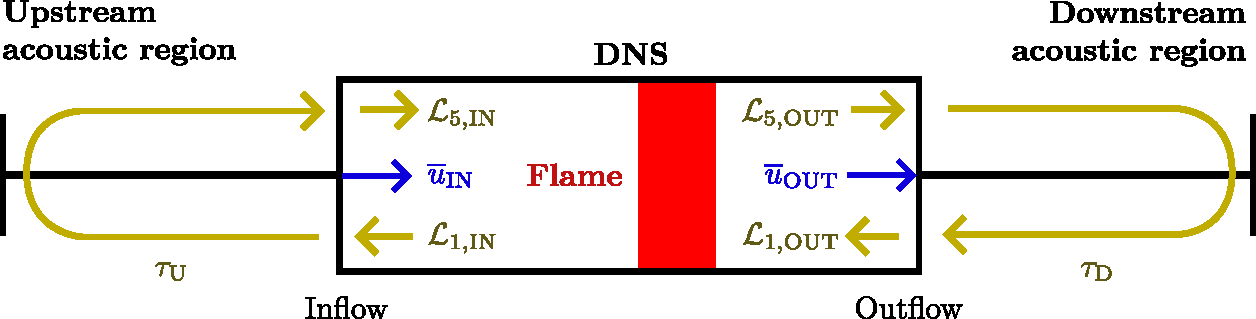
\includegraphics[scale=0.6]{assets/imgs/delay_bc_model.pdf}
\label{fig:delay-model}
\caption{MODEL OF DELAY BC. DELAY IS ONLY MODELLED VIA TIME SERIES OF L VALUES AS THEY LEAVE THE DNS DOMAIN.}
\end{figure}

\begin{figure}[t]
\centering
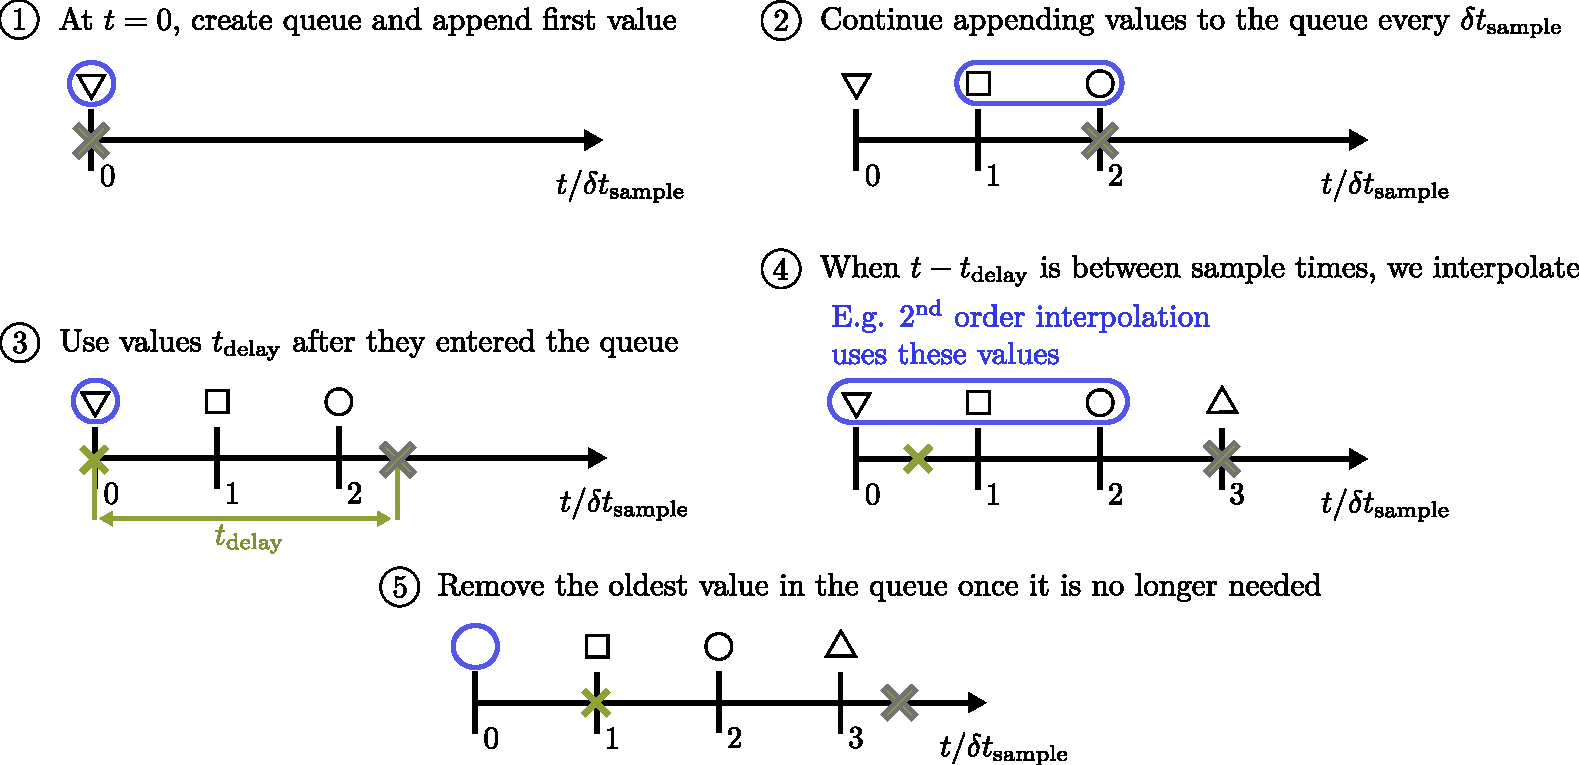
\includegraphics[scale=0.6]{assets/imgs/delay_bc_queue.pdf}
\label{fig:delay-queue}
\caption{HOW THE BOUNDARY SAMPLING AND DELAY WORK. WHAT DO SHAPES REPRESENT?? GREY CROSS IS CURRENT SIMULATION TIME, GOLD CROSS IS THAT TIME MINUS THE TIME DELAY. CHANGING TIME DELAY IS NOT SHOWN HERE.}
\end{figure}

\begin{figure}[t]
\centering
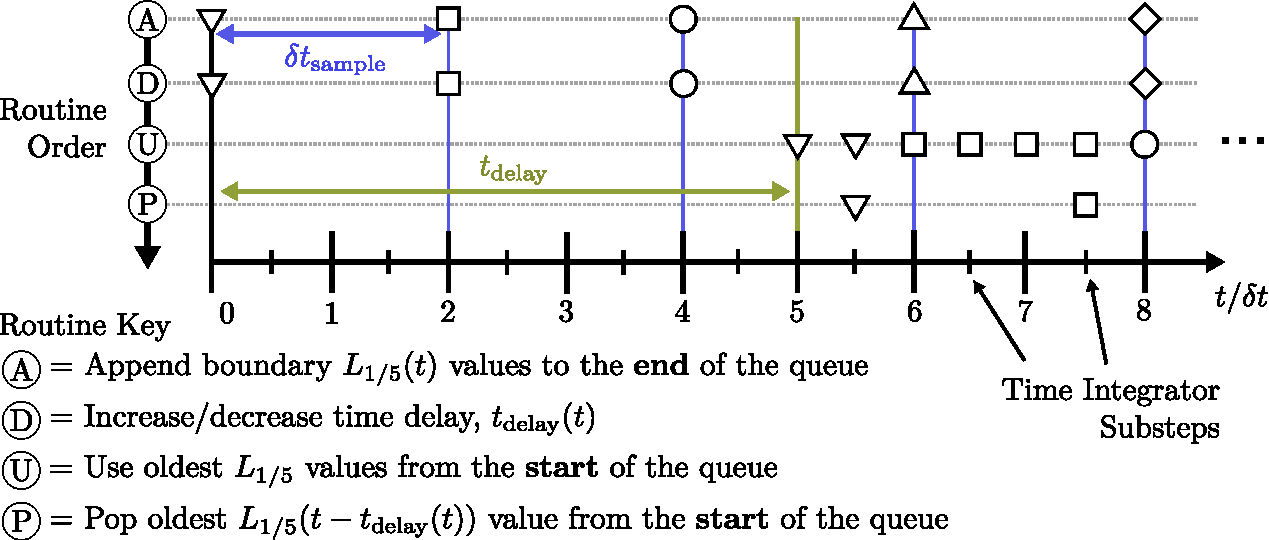
\includegraphics[scale=0.6]{assets/imgs/delay_bc_code_schematic.pdf}
\label{fig:schematic}
\caption{Schematic for delay BCs implemented into a multistage time integrator. ASSUMES CONSTANT TIME STEPS. TOP TO BOTTOM, LEFT TO RIGHT. BLUE SHOWS SAMPLE TIMES, GOLD SHOWS TIME DELAY}
\end{figure}


\begin{itemize}
\item Queues are filled with $L$ values as well as 
\end{itemize}



\subsection{Overcoming Instabilities}



\subsection{Sampling Error}






\chapter{Conclusion} \label{ch:conc}
CONCLUSIONS

\chapter{Plan For Upcoming Years} \label{ch:plan}
\section{Future Work}




\section{Planning}

\blue{Gantt Chart!!}


\printbibliography[title={References},heading=bibintoc]


\end{document}
